%Version 3.1 December 2024
% See section 11 of the User Manual for version history
%
%%%%%%%%%%%%%%%%%%%%%%%%%%%%%%%%%%%%%%%%%%%%%%%%%%%%%%%%%%%%%%%%%%%%%%
%%                                                                 %%
%% Please do not use \input{...} to include other tex files.       %%
%% Submit your LaTeX manuscript as one .tex document.              %%
%%                                                                 %%
%% All additional figures and files should be attached             %%
%% separately and not embedded in the \TeX\ document itself.       %%
%%                                                                 %%
%%%%%%%%%%%%%%%%%%%%%%%%%%%%%%%%%%%%%%%%%%%%%%%%%%%%%%%%%%%%%%%%%%%%%

\documentclass[pdflatex,sn-basic]{sn-jnl}% Springer Nature basic reference style, single-column layout

%%%% Standard Packages
%%<additional latex packages if required can be included here>

\usepackage{graphicx}%
\usepackage{multirow}%
\usepackage{amsmath,amssymb,amsfonts}%
\usepackage{amsthm}%
\usepackage{mathrsfs}%
\usepackage[title]{appendix}%
\usepackage{xcolor}%
\usepackage{textcomp}%
\usepackage{manyfoot}%
\usepackage{booktabs}%
\usepackage{listings}%
\usepackage{algorithm}%
\usepackage{algpseudocode}%
\usepackage{url}%
\usepackage{array}%
\usepackage{tabularx}%
\usepackage{makecell}%
\usepackage{float}%
\usepackage[section]{placeins}%
%%%%

% Slightly loosen table rows for readability without changing body text spacing.
\renewcommand{\arraystretch}{1.16}%
\setlength{\extrarowheight}{0.6pt}%
\newcolumntype{L}[1]{>{\raggedright\arraybackslash}p{#1}}%
\newcolumntype{C}[1]{>{\centering\arraybackslash}p{#1}}%
\newcolumntype{Y}{>{\raggedright\arraybackslash}X}%
\newcolumntype{Z}{>{\centering\arraybackslash}X}%
\newcommand{\compacttable}{\scriptsize\setlength{\tabcolsep}{2.2pt}\renewcommand{\arraystretch}{1.12}}%
\makeatletter
\g@addto@macro\UrlBreaks{\do\/\do\-\do\.}%
\makeatother
\Urlmuskip=0mu plus 1mu\relax
\hypersetup{hypertexnames=false}%

% Local readability override for author-side PDF review.
% Springer Nature's class uses a narrow two-sided text block with a binding offset;
% comment this line before submission if the journal requires the untouched template layout.
\geometry{textwidth=154mm,bindingoffset=0mm}%

\usepackage{indentfirst}%

%%%%%=============================================================================%%%%
%%%%  Remarks: This template is provided to aid authors with the preparation
%%%%  of original research articles intended for submission to journals published
%%%%  by Springer Nature. The guidance has been prepared in partnership with
%%%%  production teams to conform to Springer Nature technical requirements.
%%%%  Editorial and presentation requirements differ among journal portfolios and
%%%%  research disciplines. You may find sections in this template are irrelevant
%%%%  to your work and are empowered to omit any such section if allowed by the
%%%%  journal you intend to submit to. The submission guidelines and policies
%%%%  of the journal take precedence. A detailed User Manual is available in the
%%%%  template package for technical guidance.
%%%%%=============================================================================%%%%

\theoremstyle{thmstyleone}%
\newtheorem{theorem}{Theorem}%
\newtheorem{proposition}[theorem]{Proposition}%

\theoremstyle{thmstyletwo}%
\newtheorem{example}{Example}%
\newtheorem{remark}{Remark}%

\theoremstyle{thmstylethree}%
\newtheorem{definition}{Definition}%

\lstset{
  basicstyle=\ttfamily\footnotesize,
  backgroundcolor=\color{gray!5},
  frame=single,
  keywordstyle=\color{blue}\bfseries,
  commentstyle=\color{gray}\itshape,
  stringstyle=\color{red!60!black},
  numbers=left,
  numberstyle=\tiny\color{gray},
  breaklines=true,
  captionpos=b,
  escapeinside={(*@}{@*)}
}

\raggedbottom

\begin{document}
\articletype{RESEARCH}

\title{Evidence-Guided Crash Adjudication for LLM-assisted Fuzzing of Third-party Open-source Libraries in Connected Vehicles}

\author*[1]{\fnm{Qingguan} \sur{Gao}}\email{gaoqingguan@seu.edu.cn}

\author[1]{\fnm{Ying} \sur{Zhang}}\email{zhangying@seu.edu.cn}

\author[2]{\fnm{Letian} \sur{Sha}}\email{ltsha@njupt.edu.cn}

\author[3]{\fnm{Huiran} \sur{Yang}}\email{yanghuiran@zdcst.cn}

\affil*[1]{\orgname{School of Cyber Science and Engineering, Southeast University}, \orgaddress{\city{Nanjing}, \country{China}}}

\affil[2]{\orgname{School of Computer Science, Nanjing University of Posts and Telecommunications}, \orgaddress{\city{Nanjing}, \country{China}}}

\affil[3]{\orgname{The First Research Institute of the Ministry of Public Security}, \orgaddress{\country{China}}}

\abstract{
{\color{yellow}Connected-vehicle software relies on third-party open-source libraries, making it a relevant application setting for studying crash adjudication in LLM-assisted fuzzing.}
Advances in Large Language Models (LLMs) have increasingly automated fuzz-driver generation. Nevertheless, directly applying LLMs to raw crash reports can produce many false alerts, while case-by-case triage incurs prohibitive labor costs. To tackle this problem, we propose CrashSage, an evidence-guided framework for post-fuzzing crash adjudication in LLM-assisted fuzzing. Before final LLM analysis, CrashSage prepares crash evidence through three key designs: rule-guided crash attribution, representative selection, and crash-context reconstruction. Rule-guided crash attribution filters low-value reports and likely driver-induced crashes to improve false-alert judgment. Representative selection compares exact and stack signatures among retained reports to identify repeated crash instances and submits only selected representatives to the LLM, reducing redundant analysis. Crash-context reconstruction enriches representatives with static and runtime evidence, helping determine whether the faulty state comes from the generated driver or the target component.
{\color{yellow}Experiments on 1,217 crash reports from 14 third-party open-source libraries relevant to connected-vehicle software show that CrashSage achieves 76.54\% precision, 92.56\% recall, and an 83.79\% F1 score, while reducing LLM submissions from 1,217 to 96 (92.11\%). These results support CrashSage as a crash-adjudication aid in this application setting.}
}

\keywords{fuzz testing, crash adjudication, large language model, crash attribution, connected vehicle security}

\maketitle


\section{Introduction}
\label{sec:introduction}

Intelligent connected vehicle (ICV) systems increasingly depend on third-party open-source libraries \citep{ref1,ref2,ref3,ref4,ref32}, causing ICV software to inherit security risks from these libraries. To expose crash-inducing defects in such libraries, fuzz testing is widely adopted \citep{ref16,ref17,ref7}. Yet validating diverse third-party open-source libraries at scale still requires a large number of library-specific fuzz drivers. Recent LLM-assisted fuzzing systems attempt to ease this bottleneck by using LLMs to synthesize fuzz drivers automatically \citep{ref8,ref9,ref10,ref11,ref12}. {\color{yellow}
In this study, connected-vehicle software provides the application setting rather than a vehicle-specific prerequisite of the method, and the evaluation focuses on its third-party-library components.
}

LLM-assisted fuzzing differs from conventional component fuzzing, where the harness is usually written or reviewed by developers and is therefore treated as trusted during crash inspection. In LLM-assisted fuzzing, the generated driver is not necessarily a trusted harness. It invokes target-component APIs with mutated inputs, but it may omit required initialization, construct invalid arguments, or introduce harness-level memory errors. As a result, a crash report no longer reflects target-component behavior alone, but the interaction between the generated driver and the target component.

This difference leads to three challenges in false-alert judgment, crash localization, and efficiency. First, existing crash adjudication tends to treat crash reports as direct evidence of target-component-attributed crashes, leaving driver-induced false alerts difficult to distinguish from target-component-originated crashes. Second, existing adjudication lacks localization evidence that combines static code context and runtime context, which can lead to inaccurate crash attribution. Third, repeated crash instances triggered during fuzzing may stem from the same underlying failure pattern, but existing workflows still analyze them separately, resulting in redundant triage, localization effort, and LLM submissions.

To address this problem, we propose CrashSage, an evidence-guided crash-adjudication pipeline tailored for LLM-assisted fuzzing with untrusted generated drivers. Rather than reasoning directly over raw crash reports, CrashSage applies rule-guided crash attribution to filter low-value reports and likely driver-induced failures, uses representative selection to reduce repeated crash instances, and performs crash-context reconstruction to localize the origin and propagation of the faulty state for the selected representatives. The resulting evidence is then submitted to LLM analysis for final crash diagnosis. In this way, the LLM reasons over filtered, representative, and localized crash evidence. CrashSage is designed as a post-fuzzing triage aid that reduces the number of reports requiring detailed inspection and prepares attribution evidence for retained representative crashes. The main contributions of this paper are listed as follows.

\begin{itemize}
    \item CrashSage pipeline. We propose an evidence-guided crash-adjudication pipeline for LLM-assisted fuzzing. By preparing structured crash evidence before model reasoning, CrashSage reframes the LLM from a primary classifier over raw crash text into a final analyzer over curated execution evidence.
    \item Rule-guided crash attribution. We introduce rule-guided crash attribution over sanitizer signals and stack-frame roles. This stage filters low-value reports and likely driver-induced crashes before LLM analysis, mitigating over-attribution bias in prompt-based methods and improving false-alert judgment.
    \item Representative selection. We compare exact and stack signatures to identify repeated crash instances and retain representative crashes for subsequent LLM analysis. This selection process reduces redundant analysis while preserving the relationship between each repeated crash and its representative.
    \item Crash-context reconstruction. We reconstruct static code context and runtime context for representative crashes to trace a crash across driver and component code. By combining source locations with execution-state evidence, this stage supports crash attribution by distinguishing the visible crash site from the origin of the faulty state.
    \item Experimental evaluation. {\color{yellow}We evaluate CrashSage on 1,217 crash reports from 14 third-party open-source libraries. The full pipeline achieves 76.54\% precision, 92.56\% recall, and an 83.79\% F1 score, while reducing LLM submissions from 1,217 to 96 (92.11\%). Runtime measurements identify context reconstruction and LLM analysis as the main costs, while rule-guided attribution and representative selection remain lightweight.}
\end{itemize}

The rest of the paper is organized as follows. Section~\ref{sec:related-work} reviews related work. Section~\ref{sec:preliminaries} introduces the LLM-assisted fuzzing framework and its crash-adjudication challenges. Section~\ref{sec:approach} presents the design of CrashSage, Section~\ref{sec:evaluation} reports the evaluation, and Section~\ref{sec:conclusion} concludes the paper.


\section{Related Work}
\label{sec:related-work}

\subsection{LLM-Assisted Fuzzing}

Fuzz testing remains a standard way to expose memory-safety defects in C/C++ software, especially with sanitizer support and continuous fuzzing infrastructure \citep{ref16,ref17,ref18,ref19,ref7}. In conventional component fuzzing, the driver is usually written or reviewed by developers, so downstream analysis can treat it as part of the trusted harness. However, writing such drivers for diverse libraries and APIs requires substantial manual effort, which limits the scalability of component-level fuzzing.

Recent LLM-assisted fuzzing systems address this scalability problem by using models to infer protocol knowledge, generate inputs, synthesize fuzz drivers, and repair compilation errors. ChatAFL \citep{ref8} guides stateful protocol fuzzing with LLM-derived knowledge; FuzzGPT \citep{ref9} and TitanFuzz \citep{ref10} use LLMs for edge-case or test-input generation; Fuzz4All \citep{ref11} generalizes LLM-based input generation across languages; PromptFuzz \citep{ref13} studies prompt strategies for C/C++ fuzz-driver generation; and CKGFuzzer \citep{ref12} combines code-knowledge-graph construction with LLM-based driver generation and repair. Surveys of LLM-assisted testing likewise emphasize test generation, input synthesis, and repair \citep{ref27}. These systems lower driver-construction cost, but their main optimization target remains the upstream fuzzing workflow. Once a generated driver compiles and produces crashes, crash reports are usually treated as fuzzing outcomes rather than as evidence that must be adjudicated under an untrusted-harness assumption. As a result, existing LLM-assisted fuzzing work does not directly address whether a crash report reflects a driver-induced false alert or a target-component-originated crash.

\subsection{Automated Crash Diagnosis and Reasoning}

Given the post-fuzzing analysis gap left by LLM-assisted fuzzing, a natural question is whether existing crash diagnosis techniques can resolve the resulting crash reports. Early automated diagnosis methods relied on stack-trace signatures and heuristic rules for clustering, localization, and duplicate detection. Igor \citep{ref21} clusters fuzz crashes by root cause; FuzzerAid \citep{ref22} groups crashes using learned fault signatures; CrashLocator \citep{ref23} localizes crashing faults from crash stacks; FaST \citep{ref24} aligns stack traces efficiently; and ReBucket \citep{ref25} clusters duplicate crash reports using call-stack similarity. Related methods enrich crash reports with source, execution, or explanation-oriented evidence: DeepAnalyze \citep{ref14} localizes crashing faults at scale, CrashTranslator \citep{ref15} reconstructs executable scenarios from stack traces, and Better Debugging \citep{ref20} combines static analysis with LLMs for explainable crash localization.

These techniques provide useful clustering and localization support, but they are most effective when crash evidence is stable and the harness is trusted. This assumption weakens under LLM-generated fuzz drivers. Analyses that do not explicitly localize the failure across driver and component code can mistake a component-visible crash site for a component-originated failure. Localization-oriented methods alleviate part of this ambiguity by recovering static code context, but existing execution enrichment is not designed to bind replay-consistent runtime context to driver/component attribution. Consequently, it may not reveal the runtime values, pointer states, or object states that determine whether the failure originates from driver-side construction or target-component behavior. Likewise, crash clustering can group repeated reports, but it does not by itself decide which representative should receive expensive LLM analysis or how duplicate reports should inherit the representative diagnosis.

LLM-based vulnerability reasoning appears to offer richer semantic judgment for this setting. CVE-LLM enriches vulnerability evaluation with cybersecurity ontologies \citep{ref28}, while AutoCVSS studies prompting, few-shot examples, and retrieval-augmented generation for CVSS prediction \citep{ref29}. However, these systems typically reason over curated vulnerability descriptions or structured security context, whereas LLM-assisted fuzzing often yields short crash reports from automatically generated drivers. Direct prompting over such reports lacks the structured semantics assumed by vulnerability-reasoning systems and can amplify over-attribution.

Overall, existing work leaves three gaps for LLM-assisted fuzzing crash adjudication. It does not reliably support false-alert judgment when sanitizer evidence mixes driver behavior with target-component behavior. It lacks attribution-oriented localization that combines static code context and runtime context, making it difficult to determine whether a failure propagates from the generated driver or originates within the target component. It also leaves efficiency concerns when repeated crash instances caused by the same underlying failure pattern are analyzed through separate LLM submissions. This motivates a pipeline that combines rule-guided crash attribution, representative selection, crash-context reconstruction, and LLM-based semantic reasoning before final crash diagnosis.



\section{LLM-Assisted Fuzzing Framework and Challenges}
\label{sec:preliminaries}

\subsection{LLM-Assisted Fuzzing Framework}

Figure~\ref{fig:fig1} illustrates the overall workflow of the LLM-assisted fuzzing framework considered in this work. The framework automates the process from modeling component APIs to generating fuzz drivers and collecting crash reports, and consists of three stages: API knowledge modeling, driver generation, and crash-oriented fuzzing \citep{ref12}.

API knowledge modeling. This stage first extracts the APIs to be tested from open-source components. Static feature extraction then collects key information about the target APIs and identifies their relationships. The extracted information is organized into an API knowledge graph, which provides structured API knowledge for subsequent combination planning and driver generation \citep{ref12}.

Driver generation. The combination agent summarizes the target APIs and uses the API knowledge graph to plan API combinations. Each planned combination, together with the corresponding API source code and summaries, is provided to the driver generation agent, which synthesizes a fuzz driver that invokes the selected APIs \citep{ref8,ref12,ref13}.

Crash-oriented fuzzing. For each generated driver, the seed-generation agent produces initial seeds. The fuzzing engine iteratively mutates these seeds and executes the driver in an attempt to trigger crashes. When a crash occurs, the sanitizer records the failure and exports the corresponding crash report for subsequent crash adjudication \citep{ref16,ref17,ref18,ref19}.

\begin{figure}[H]
\centering
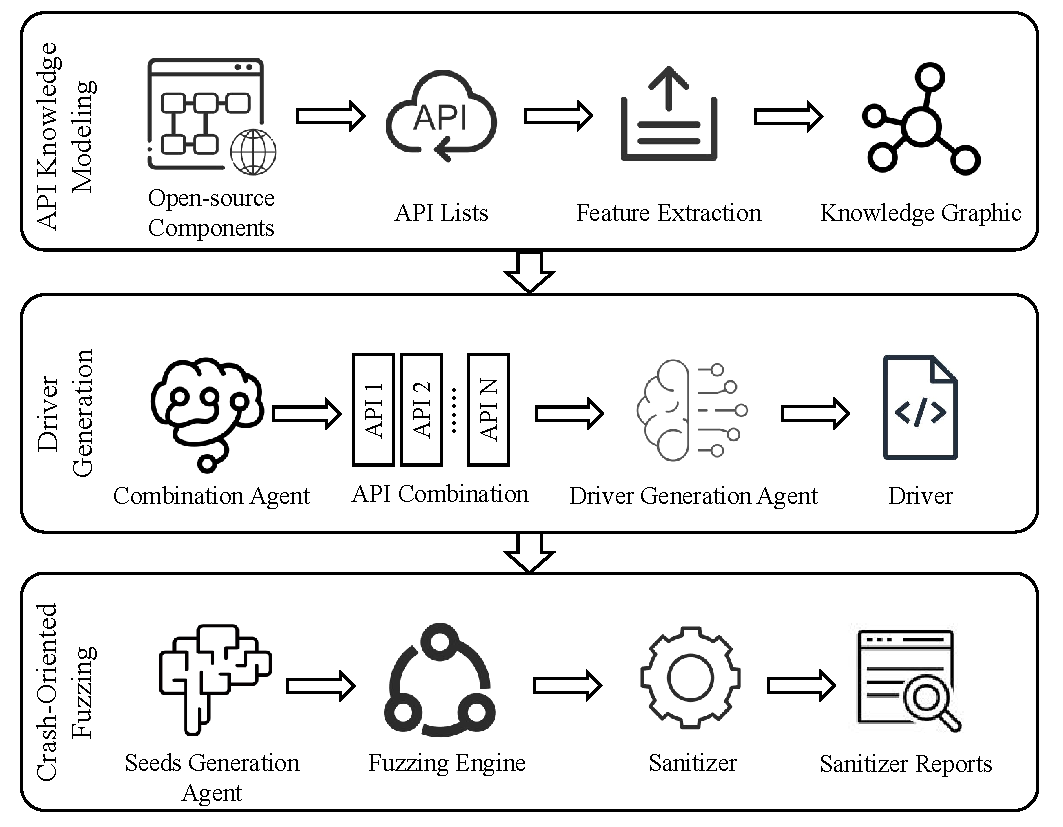
\includegraphics[width=0.75\linewidth]{figures/fig1.pdf}
\caption{Overview of the LLM-assisted fuzzing framework.}
\label{fig:fig1}
\end{figure}

\subsection{Challenges Statement}

Unlike conventional fuzzing, LLM-assisted fuzzing cannot assume that the generated driver is a trusted harness \citep{ref12,ref13}. A reported crash may result from the target component, the generated driver, or their interaction under a mutated input. Consequently, the crash report alone may not provide sufficient evidence for reliable post-fuzzing analysis. This setting raises three challenges: false-alert judgment, crash localization, and efficiency.

False-alert judgment. An LLM-generated driver may violate implicit API contracts by omitting required initialization, constructing inconsistent object states, or passing invalid argument combinations. Such misuse can trigger a failure while execution is inside the target component, causing the sanitizer stack trace to contain component frames even when the underlying fault originates from the driver. The presence of a component frame therefore does not by itself establish target-component attribution. Distinguishing driver-induced failures from target-component-originated crashes is difficult because a raw report records where the failure becomes observable, but does not explicitly identify which side violated the required execution contract.

Efficiency. LLM-assisted fuzzing repeatedly mutates related inputs, so many crashing inputs may exercise the same underlying failure pattern. Different generated drivers may also reach that failure pattern through distinct API combinations or call paths. These executions can produce reports that differ in addresses, stack depth, or intermediate frames despite sharing one root cause \citep{ref21,ref22,ref25}. Treating every report as an independent case leads to repeated inspection and redundant LLM submissions, making crash adjudication increasingly expensive as the number of generated drivers and crashing inputs grows.

Crash localization. Existing prompt-based analysis commonly reasons over raw crash reports without explicitly localizing the failure across the generated driver and the target component. Because a driver-constructed invalid state may become observable only after entering component code, the visible crash frame can be mistaken for evidence that the open-source supply-chain component caused the failure. Localization information is therefore necessary not only to identify a suspicious statement, but also to determine where the faulty state originates and how it reaches the crash site \citep{ref14,ref15,ref20,ref23}. However, existing localization evidence is dominated by static code context, while runtime context is not systematically incorporated into driver/component attribution. Static code context cannot expose the concrete values, pointer states, or object states involved in the failing execution, leaving the propagation of the faulty state incomplete and crash attribution uncertain.


\section{Approach}
\label{sec:approach}

\subsection{CrashSage Design Overview}
\label{subsec:problem-overview}

In this section, we present the system design of CrashSage, an evidence-guided crash-adjudication framework for LLM-assisted fuzzing. CrashSage is designed to improve post-fuzzing crash adjudication when automatically generated fuzz drivers cannot be treated as trusted harnesses. Its primary objective is to prepare structured evidence that supports attribution-oriented localization, remove repeated crash instances, and retain auditable inputs before final LLM reasoning. Through this pipeline, CrashSage supports false-alert judgment, crash localization, and efficient analysis of repeatedly triggered crashes.

Figure~\ref{fig:three-mechanism-design} illustrates the workflow of CrashSage and aligns the three challenges with the corresponding processing stages. Initially, \emph{rule-guided crash attribution} addresses false-alert judgment by distinguishing noise and likely driver-induced crashes from cases that require further target-component analysis. It normalizes crash reports and applies rule-based preliminary screening over sanitizer signals and stack-frame roles, producing filtered normalized crash reports for the following stages. Next, \emph{representative selection} addresses efficiency by avoiding repeated analysis of crashes that follow the same underlying failure pattern. It constructs exact and stack signatures from the normalized sanitizer evidence, verifies signature matches, maps repeated crashes to an existing representative, and retains unmatched crashes in the selected crash set. CrashSage then performs \emph{crash-context reconstruction} to enrich these selected representatives with static code context and replay-consistent runtime context, helping determine where an invalid state originates and how it propagates to the visible crash site. Finally, \emph{LLM analysis} completes the semantic diagnosis by combining each representative crash's normalized crash report, triage label, and reconstructed context to determine its type, cause, location, triggering condition, and severity.


\begin{figure}[H]
\centering
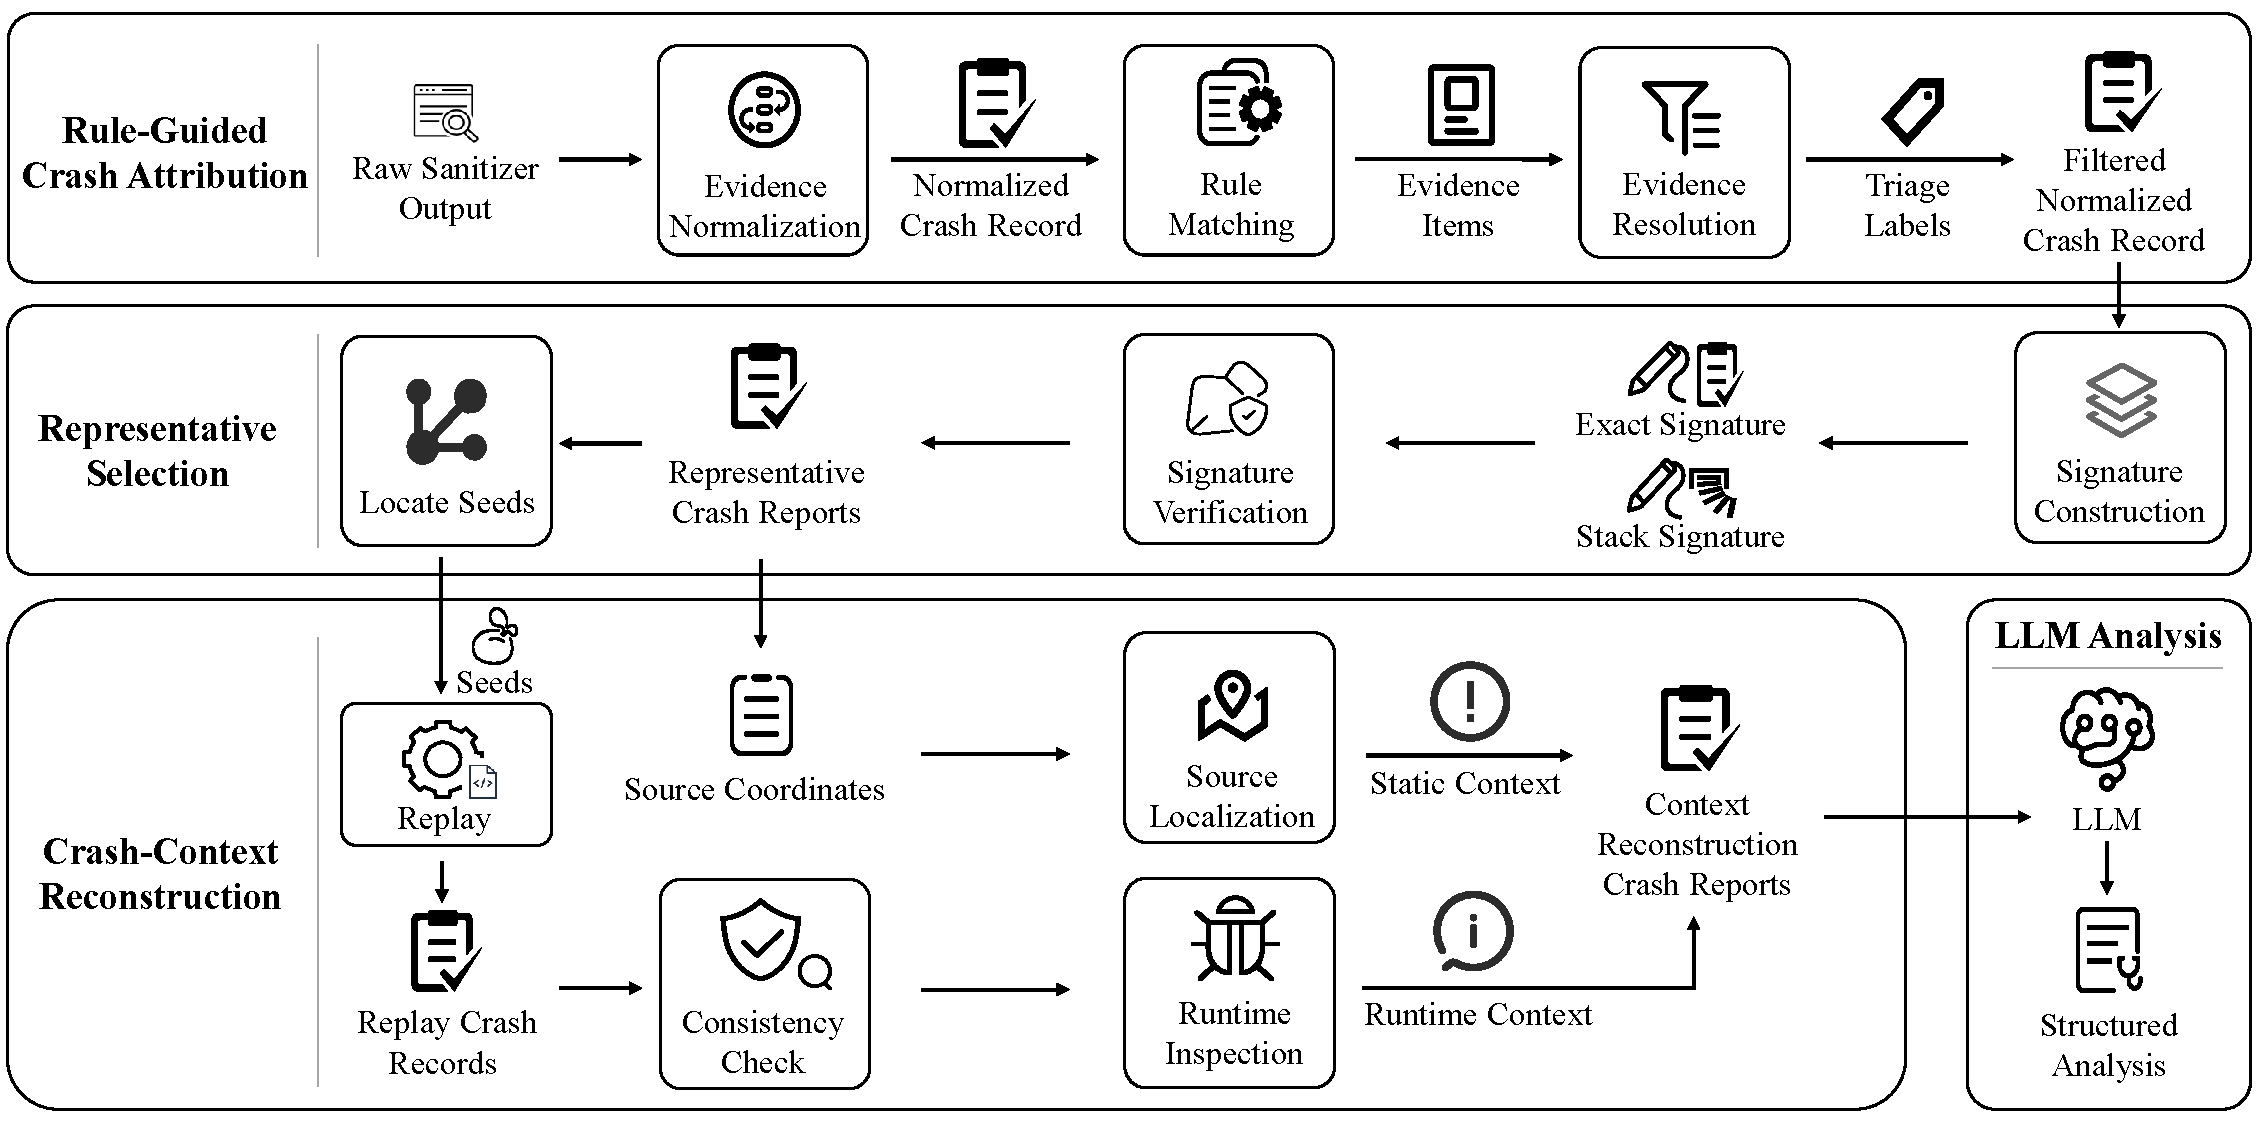
\includegraphics[width=0.75\linewidth]{figures/fig2.pdf}
\caption{Multi-stage crash-adjudication pipeline combining rule-guided crash attribution, representative selection, crash-context reconstruction, and LLM analysis.}
\label{fig:three-mechanism-design}
\end{figure}


\subsection{Rule-Guided Crash Attribution}
\label{subsec:rule-guided-attribution}

Rule-guided crash attribution is the first stage of CrashSage and addresses the false-alert judgment challenge.
It consists of sanitizer evidence normalization and rule-based preliminary screening.
The former converts raw sanitizer output into a normalized crash report, while the latter assigns a triage label that determines whether the crash is filtered.

\subsubsection{Sanitizer Evidence Normalization}
Crash reports contain substantial redundant information that is not directly useful for subsequent crash adjudication. 
CrashSage normalizes each raw crash report into a normalized crash report that retains the information required by subsequent stages.
Table~\ref{tab:sanitizer-normalized-fields} summarizes the normalized field groups.

\begin{itemize}
    \item Failure identity describes the crash report type and its failure category.
    \item Crash-site metadata records the immediate low-level crash information, such as the failing address or access behavior, when it is available.
    \item Severity and dedup cues provide sanitizer- or fuzzer-generated hints that help prioritize and compare crash reports.
    \item Structured stack trace converts the raw call stack into ordered frames for later role modeling.
    \item Project anchor identifies the first visible connection between the crash trace and the target-component source code.
    \item Reproduction and status hints preserve crash-input clues and special execution states that may affect filtering or replay.
\end{itemize}

\begin{table}[t]
\caption{Key field groups in the normalized crash report}
\label{tab:sanitizer-normalized-fields}
\centering
\compacttable
\setlength{\tabcolsep}{4.0pt}
\renewcommand{\arraystretch}{1.10}
\begin{tabular*}{\linewidth}{@{\extracolsep{\fill}}ll}
\toprule
Field Group & Representative Extracted Fields \\
\midrule
Failure identity & \texttt{sanitizer\_type}, \texttt{bug\_type}, \texttt{summary} \\
Crash-site metadata & \texttt{crash\_address}, \texttt{pc}, \texttt{access\_type} \\
Severity and dedup cues & \texttt{scariness\_score}, \texttt{scariness\_desc}, \texttt{dedup\_token} \\
Structured stack trace & ordered \texttt{frames} with function, file, line, and address \\
Project anchor & \texttt{first\_in\_project\_frame}, \texttt{first\_in\_project\_function} \\
Reproduction and status hints & \texttt{artifact\_path\_hint}, \texttt{base\_unit\_hash}, special-condition flags \\
\botrule
\end{tabular*}
\end{table}
\FloatBarrier

\subsubsection{Rule-Based Preliminary Screening}
Screening begins by matching the function name, file path, and position of each frame in the \texttt{structured stack trace} against predefined project, driver, and runtime patterns.
Frames without sufficient matching evidence remain \emph{unclassified}.

\begin{table}[!htbp]
\caption{Stack-frame role classification used by CrashSage}
\label{tab:stack-frame-roles}
\centering
\scriptsize
\setlength{\tabcolsep}{4.0pt}
\renewcommand{\arraystretch}{1.10}
\begin{tabular*}{\linewidth}{@{\extracolsep{\fill}}ll}
\toprule
Role & Meaning \\
\midrule
project & Stack frames in the target-component source code. \\
driver & Stack frames related to the fuzz driver. \\
runtime & Runtime-library frames, including libFuzzer, sanitizers, LLVM runtime, libc, etc. \\
unclassified & Frames that cannot be classified reliably but are not obvious runtime frames. \\
\botrule
\end{tabular*}
\end{table}
\FloatBarrier

Table~\ref{tab:stack-frame-roles} summarizes these roles. Frame ownership alone is not sufficient for false-alert judgment.
A crash trace can involve target-component frames, generated-driver frames, and runtime frames at the same time, while the frame where the sanitizer reports the failure may not be the frame that best explains the origin of the crash.
CrashSage therefore applies a set of deterministic rules over the ownership and position of stack frames to infer whether the crash is more consistent with noise, a driver-induced failure, or a target-component crash.

Before listing the rules, we define the following notations.
Let \(S=\langle f_1,\ldots,f_n\rangle\) denote the structured stack trace, ordered from the top crashing frame to lower caller frames.
Let \(F_P\), \(F_D\), and \(F_N\) denote the sets of project frames, driver frames, and non-runtime frames, respectively, where \(F_N=F_P\cup F_D\cup F_U\) and \(F_U\) is the set of unclassified frames.
CrashSage computes the driver-frame ratio
\begin{equation*}
R_D=\frac{|F_D|}{\max(|F_N|,1)} ,
\end{equation*}
corresponding to \texttt{Driver\_Frame\_Ratio}.
Runtime frames are excluded from this ratio because they mainly reflect sanitizer and libFuzzer control flow.
Let \(h_D\) denote the top-stack depth inspected for driver evidence, \(\theta_D\) the driver-frame-ratio threshold, \(m_P\) the maximum number of project frames treated as shallow project involvement, and \(\theta_S\) the sanitizer-severity threshold.

CrashSage sets these parameters through an evidence-boundary design strategy that maps each value to an interpretable stack or sanitizer signal.
The parameter \(h_D\) defines the near-crash stack region used for driver-evidence inspection, \(\theta_D\) defines the driver-dominance level in the attribution-relevant non-runtime stack, \(m_P\) defines the amount of project-code involvement treated as shallow API-boundary execution, and \(\theta_S\) defines the sanitizer-severity level used to retain project-frame SEGV/null-dereference reports.

For \(h_D\), CrashSage sets \(h_D=3\) because a three-frame window corresponds to the crash frame, the direct caller, and the caller that usually reflects the immediate driver-side invocation context.
This value keeps the check centered on the local failure path where argument construction, API invocation, and first observable faulty use are most directly represented.
For \(\theta_D\), CrashSage sets \(\theta_D=0.8\), using a four-fifths majority as the driver-dominance criterion over non-runtime frames.
This value requires driver evidence to occupy a clearly dominant share of the attribution-relevant stack before assigning \texttt{likely\_driver\_bug}, making the label depend on stack-level concentration rather than an isolated driver frame.
For \(m_P\), CrashSage sets \(m_P=2\) because shallow API-boundary execution often includes the target entry function and one adjacent helper, initialization, creation, setup, or parsing frame.
This value captures brief project-code contact during driver-constructed calls while distinguishing it from deeper target-component execution paths.
For \(\theta_S\), CrashSage sets \(\theta_S=10\) as the high-severity sanitizer threshold for SEGV/null-dereference reports.
This value retains reports when the sanitizer signal indicates severe invalid memory access and the stack simultaneously provides project-frame evidence for target-component analysis.

These values are fixed before evaluating the crash reports, providing a stable and reproducible configuration for the rule-guided attribution stage. The remaining rule signals also come from the normalized crash report.
Timeout, \texttt{ALARM}, out-of-memory, LSan-only, and deadly-signal flags are extracted from sanitizer or libFuzzer status lines, while \texttt{SCARINESS} comes from the sanitizer severity line.
Table~\ref{tab:triage-rule-groups} summarizes the 13 deterministic rules, their predicates, and their preliminary output labels.
These labels express the direction supported by the available evidence rather than a final vulnerability verdict.

\begin{table}[t]
\caption{Rules used for crash attribution}
\label{tab:triage-rule-groups}
\centering
\compacttable
\setlength{\tabcolsep}{2.4pt}
\renewcommand{\arraystretch}{1.10}
\begin{tabularx}{\linewidth}{C{0.08\linewidth} C{0.08\linewidth} Y L{0.19\linewidth}}
\toprule
Group & Rule & Deterministic Predicate & Output Label \\
\midrule
NF & R1 & \(F_N=\emptyset \land \texttt{deadly\_signal}\) & \texttt{noise} \\
NF & R2 & Timeout or \texttt{ALARM} marker appears & \texttt{noise} \\
NF & R3 & Out-of-memory marker appears & \texttt{noise} \\
NF & R4 & LSan-only report without crashing execution & \texttt{noise} \\
\midrule
DQ & R5 & \(\texttt{use\_of\_uninitialized\_value}\) with a driver frame in the top-\(h_D\) stack frames & \texttt{likely\_driver\_bug} \\
DQ & R6 & \(R_D\ge \theta_D\) & \texttt{likely\_driver\_bug} \\
DQ & R7 & Project init/option/parse function appears near the driver boundary & \texttt{likely\_driver\_bug} \\
DQ & R8 & \(\texttt{stack\_buffer\_overflow}\) with the first non-runtime frame in driver code & \texttt{likely\_driver\_bug} \\
DQ & R9 & \(F_N=F_D \land F_P=\emptyset\) & \texttt{likely\_driver\_bug} \\
DQ & R10 & \(|F_P|\le m_P\) and project function matches init/create patterns & \texttt{likely\_driver\_bug} \\
\midrule
TC & R11 & Memory-safety crash with at least one project frame & \texttt{target\_crash} \\
TC & R12 & SEGV/null-dereference with \(\texttt{SCARINESS}\ge \theta_S\) and project frame evidence & \texttt{target\_crash} \\
\midrule
LE & R13 & Assertion, abort, or \texttt{ABRT} originates in project code & \texttt{needs\_review} \\
\botrule
\end{tabularx}
\vspace{2pt}
{\raggedright\scriptsize \textit{Note.} NF: noise filtering; DQ: driver-quality detection; TC: target-component attribution indication; LE: logic-error indication. \(F_N\), \(F_D\), and \(F_P\) denote non-runtime, driver, and project frame sets, respectively.\par}
\end{table}

\begin{itemize}
    \item R1. A \texttt{deadly\_signal} marker confirms abnormal termination, but the absence of non-runtime frames leaves no project or driver location for attribution. The report is therefore labeled \texttt{noise} because it provides no inspectable evidence for the subsequent analysis.
    \item R2. Timeout and \texttt{ALARM} markers indicate that execution exceeded its time limit, without providing sanitizer evidence for a memory-access crash. Such reports are labeled \texttt{noise} because they do not provide crash evidence for component attribution.
    \item R3. An out-of-memory marker records resource exhaustion, which may depend on allocation demand or execution limits and does not identify a specific faulty access. The rule therefore assigns \texttt{noise} rather than attributing the condition to either the driver or the target component.
    \item R4. An LSan-only report identifies unreleased allocations at process exit but contains no crashing instruction, signal, or abort. Because the rule-guided stage concerns the origin of crashes, this report is labeled \texttt{noise}.
    \item R5. An uninitialized-value report indicates that data was consumed before receiving a valid value. When driver frames occur within the top \(h_D\) frames, the first observable use is close to driver-side execution, so the available evidence supports \texttt{likely\_driver\_bug}.
    \item R6. After runtime frames are removed, \(R_D\ge \theta_D\) means that driver frames account for the specified dominant share of the attribution-relevant stack. Because the observable crash path is concentrated in the generated harness, the rule assigns \texttt{likely\_driver\_bug}.
    \item R7. Initialization, option-processing, and parsing functions near the driver boundary are commonly reached while the generated driver constructs objects and prepares API arguments. When project involvement remains at this boundary, the evidence favors invalid driver-side setup over target-component-originated execution, leading to \texttt{likely\_driver\_bug}.
    \item R8. For a stack-buffer overflow, the first non-runtime frame identifies the function whose active stack object exceeds its boundary. If this frame belongs to the driver, the overflowing object is localized to driver-side execution, so the rule assigns \texttt{likely\_driver\_bug}.
    \item R9. If every non-runtime frame belongs to the driver and no project frame is present, the trace contains no observable evidence that execution reached target-component code. The crash is therefore labeled \texttt{likely\_driver\_bug}.
    \item R10. At most \(m_P\) project frames limited to initialization or creation functions indicate shallow component involvement during API setup rather than an internal target execution path. This pattern is treated as \texttt{likely\_driver\_bug} because the evidence primarily reflects how the generated driver configured the call.
    \item R11. A sanitizer-reported memory-safety crash with at least one project frame establishes that the erroneous execution reached target-component code. The rule labels it \texttt{target\_crash} so that it is retained as a target-component candidate for subsequent stages, rather than making the final attribution decision in the rule-guided stage.
    \item R12. A severe SEGV or null dereference indicates an invalid memory access, while the presence of project frames anchors that access in target-component execution. Their combination supports the preliminary label \texttt{target\_crash} and retains the crash for localization.
    \item R13. A project-origin assertion, abort, or \texttt{ABRT} identifies the component location that terminates execution, but the report alone cannot distinguish a driver violation of an API precondition from a violated internal invariant. The rule therefore assigns \texttt{needs\_review} rather than attributing the crash to either side.
\end{itemize}

Because the rules are evaluated independently, CrashSage resolves their evidence items in the order \texttt{noise}, \texttt{likely\_driver\_bug}, \texttt{target\_crash}, and \texttt{needs\_review}.
The first matched label in this order becomes the triage label; if no rule matches, the crash is assigned \texttt{needs\_review} by default.
This procedure removes reports without usable crash evidence and generated-driver crashes before retaining target-component candidates and ambiguous cases for further analysis.

Crashes labeled \texttt{noise} or \texttt{likely\_driver\_bug} are filtered, whereas those labeled \texttt{target\_crash} or \texttt{needs\_review} are kept as retained normalized crash reports for representative selection.
For a crash \(c\), let \(\mathcal{N}(c)\) denote its normalized crash report and \(y(c)\) denote its triage label.
The output of rule-guided crash attribution is the pair \(\langle\mathcal{N}(c),y(c)\rangle\), which serves as the input to the subsequent stage.


\subsection{Representative Selection}

Large-scale fuzzing often produces many crash instances that differ in inputs or generated drivers but follow the same underlying failure pattern.
Representative selection reduces this repeated analysis cost by comparing exact and stack signatures and forwarding only non-duplicate representatives to the later LLM stage.

Let \(\mathcal{C}=\{c_1,\ldots,c_n\}\) denote the set of crashes retained after rule-guided crash attribution.
For each crash \(c\), let \(S_c\) denote its structured stack trace following the definition of \(S\) in Section~\ref{subsec:rule-guided-attribution}, and let \(d(c)\) denote the sanitizer deduplication token.
Let \(b(c)\) denote the sanitizer bug type extracted from \(\mathcal{N}(c)\), and let \(\ell(c)\) denote the crash-site source location derived from the crash-site metadata or resolved frame location when available.
Let \(\bot\) denote an unavailable value.
The sequence \(s(c)\) is the ordered non-runtime key-frame subsequence derived from \(S_c\).
Runtime frames are excluded from \(s(c)\) because they usually describe sanitizer, libFuzzer, or libc control flow rather than the project-driver execution path.

Exact signature. The exact signature targets crashes with the same sanitizer-provided identity or the same resolved crash site.
CrashSage computes
\begin{equation*}
\sigma_{\mathrm{exact}}(c)=
\begin{cases}
H(d(c)), & d(c)\neq \bot,\\
H\bigl(b(c),\ell(c),\mathrm{top}(s(c))\bigr), & d(c)=\bot \land \ell(c)\neq \bot \land |s(c)|>0,\\
\bot, & \text{otherwise},
\end{cases}
\end{equation*}
where \(H(\cdot)\) is a stable hash function and \(\mathrm{top}(s(c))\) denotes the first frame in the non-runtime key-frame sequence.
The exact-signature match between two crashes is defined as
\begin{equation*}
M_{\mathrm{exact}}(c_i,c_j)=
\mathbb{I}\bigl[
\sigma_{\mathrm{exact}}(c_i)\neq \bot
\land \sigma_{\mathrm{exact}}(c_i)=\sigma_{\mathrm{exact}}(c_j)
\bigr].
\end{equation*}
Here, \(M_{\mathrm{exact}}(c_i,c_j)=1\) represents the strongest duplicate match.
The condition holds either because both crashes expose the same sanitizer deduplication token \(d(c)\), or because the normalized fields \(b(c)\), \(\ell(c)\), and \(\mathrm{top}(s(c))\) agree.
In the latter case, the two reports have the same sanitizer crash class, the same localized crash-site anchor such as file, line, and function, and the same first project/driver frame after runtime frames are removed.

\begin{algorithm}[H]
\caption{Representative Selection}
\label{alg:representative-selection}
\begin{algorithmic}
\Require retained crashes \(\mathcal{C}=\langle c_1,\ldots,c_n\rangle\) in discovery order
\Ensure selected crash set \(\mathcal{R}\) and duplicate mapping \(\mathcal{L}\)
\State \(\mathcal{R}\gets\varnothing\), \(\mathcal{L}\gets\varnothing\)
\For{\(c_i\in\mathcal{C}\)}
    \State \(r^\ast\gets\bot\)
    \For{\(r\in\mathcal{R}\)}
        \If{\(M(c_i,r)=1\)}
            \State \(r^\ast\gets r\)
            \State \textbf{break}
        \EndIf
    \EndFor
    \If{\(r^\ast\neq\bot\)}
        \State \(\mathcal{L}\gets\mathcal{L}\cup\{(c_i,r^\ast)\}\)
    \Else
        \State \(\mathcal{R}\gets\mathcal{R}\cup\{c_i\}\)
    \EndIf
\EndFor
\State \Return \((\mathcal{R},\mathcal{L})\)
\end{algorithmic}
\end{algorithm}

Stack signature. The stack signature targets crashes whose crash-site anchors differ but whose project-driver call paths are identical.
Let \(p_k(c)\) denote the ordered sequence obtained by taking the first \(\min(k,|s(c)|)\) frames from \(s(c)\), preserving the original stack order from the top crashing frame to lower caller frames.
Here, \(k\) is a fixed prefix length used consistently for all crashes.
CrashSage builds a stack signature from this bounded prefix:
\begin{equation*}
\sigma_{\mathrm{stack}}(c)=H\bigl(b(c),p_k(c)\bigr).
\end{equation*}
The bug type is kept in the signature to avoid treating different sanitizer crash classes that happen to pass through similar functions as duplicates.
The bounded prefix of the non-runtime stack captures the driver-to-project execution path that reaches the crash.
The stack-signature match is defined as
\begin{equation*}
M_{\mathrm{stack}}(c_i,c_j)=
\mathbb{I}\bigl[
\sigma_{\mathrm{stack}}(c_i)=\sigma_{\mathrm{stack}}(c_j)
\bigr].
\end{equation*}
Here, \(M_{\mathrm{stack}}(c_i,c_j)=1\) represents a duplicate match based on the retained call path rather than on an identical crash-site anchor.
The equality of \(\sigma_{\mathrm{stack}}\) requires the same \(b(c)\) and the same bounded prefix \(p_k(c)\), where \(p_k(c)\) is built from the ordered non-runtime frames in \(s(c)\).
Thus, the two crashes are treated as duplicates when their normalized stack evidence shows the same sanitizer crash class and the same leading project/driver frame sequence, even if the reported line number, resolved crash location, or exact sanitizer token is unavailable or slightly different.

CrashSage evaluates the two match predicates in the order of exact and stack matching, which corresponds to signature verification in Figure~\ref{fig:three-mechanism-design}.
For a pair of crashes, stack matching is evaluated only when exact matching does not produce a match.
The resulting duplicate decision is
\begin{equation*}
M(c_i,c_j)=
M_{\mathrm{exact}}(c_i,c_j)
\lor M_{\mathrm{stack}}(c_i,c_j).
\end{equation*}

CrashSage processes the retained crashes in discovery order and compares each crash with the representatives selected so far.
A matched crash is linked to the corresponding representative, whereas an unmatched crash becomes a new representative.
Algorithm~\ref{alg:representative-selection} summarizes this procedure.

The primary output of representative selection is the selected crash set \(\mathcal{R}\).
The accompanying mapping \(\mathcal{L}\) records each duplicate--representative pair \((c_i,r)\), indicating that \(c_i\) matches and reuses the analysis result of representative \(r\).

\subsection{Crash-Context Reconstruction}

After representative selection, the selected crash representatives still require relevant localization evidence to refine the attribution.
A component frame identifies where a failure becomes visible, but it does not establish whether the faulty state originates in the generated driver or the target component.
Crash-context reconstruction addresses this gap through static code context reconstruction and runtime context reconstruction.
Static code context reconstruction maps the driver-to-component call path to source code, while runtime context reconstruction recovers the execution state needed to explain how the failure propagates along that path.
Together, they turn an isolated sanitizer crash label into attribution-oriented execution evidence for LLM adjudication of the selected representatives.

\subsubsection{Static Code Context Reconstruction}
Static code context reconstruction localizes selected project and driver frames in a representative crash report to source files and extracts the surrounding source-code context.
CrashSage first maps each selected frame to a local file, function, and line number using the reported source coordinates.
Based on these locations, it extracts bounded code windows around the crash-site frame and relevant call-chain frames, preserving the local statements before and after each key frame.
These code windows provide source-level evidence for inspecting the crashing operation and tracing how the fuzz input moves from the generated driver into the target API and toward the crash site.
However, static code context alone cannot determine the concrete values and object states present in the failing execution.

\subsubsection{Runtime Context Reconstruction}
Runtime context reconstruction complements static code context reconstruction by recovering execution-state evidence that static code alone cannot provide, including variable values, pointer states, and memory-related conditions at the crash point.
This evidence helps determine whether an invalid state is constructed by the driver and propagated into component code or produced within the component itself.
CrashSage uses \texttt{artifact\_path\_hint} or \texttt{base\_unit\_hash} in the normalized crash report to locate the triggering seed and stage an isolated copy for replay.

Replaying the seed is necessary to observe the execution state at the crash point.
However, environmental differences, timing-dependent behavior, uninitialized state, or external resources may cause the same seed to produce a different crash.
CrashSage therefore parses the replayed crash report into a replay-produced normalized crash record and verifies its consistency before collecting runtime context.
To bind the replay result to the representative crash, CrashSage builds a replay key
\begin{equation*}
\kappa(c)=\langle b(c), \ell(c), s(c) \rangle ,
\end{equation*}
where \(b(c)\) corresponds to the \texttt{bug\_type} field of crash report \(c\), \(\ell(c)\) denotes the crash-site source location derived from the crash-site metadata or resolved frame location when available, and \(s(c)\) denotes the ordered non-runtime key-frame sequence derived from the structured stack trace \(S\).
Let \(c_0\) denote the original normalized crash report and \(c_r\) denote the replay-produced crash record.
CrashSage regards their replay keys as compatible, denoted by \(\kappa(c_r)\simeq\kappa(c_0)\), when
\begin{equation*}
b(c_r)=b(c_0) \land s(c_r)=s(c_0) \land
\bigl(\ell(c_0)=\bot \lor \ell(c_r)=\ell(c_0)\bigr),
\end{equation*}
where \(\bot\) denotes an unavailable value in the corresponding field.
Only a replay satisfying this condition is treated as consistent with the representative crash and used for runtime inspection.

For a replay-consistent crash, CrashSage invokes GDB as the runtime inspection tool.
The bounded GDB run records the reproduced backtrace and crash frame, together with selected registers, function arguments, and local variables from the frames nearest to the crash site.
These fields can help reveal state that static code context cannot provide, such as whether a pointer is null, whether a size variable is inconsistent with a buffer, or whether an object has an invalid state before the crashing operation. Algorithm~\ref{alg:runtime-context} summarizes this reproduction-gated runtime context reconstruction procedure. The detailed organization of the evidence produced by crash-context reconstruction is presented in Table~\ref{tab:reconstruction-output-fields}.

\textsc{LocateSeed}, \textsc{StageSeed}, \textsc{ReplayAndParse}, and \textsc{CollectDebugContext} correspond to seed recovery, isolated replay preparation, replay-output parsing, and GDB-based bounded runtime-state collection, respectively.
For each representative crash \(c\in\mathcal{R}\), the output \(C_{\mathrm{recon}}(c)\) contains static code context, optional runtime context, and a status \(\rho\) indicating the outcome of seed recovery, replay matching, and GDB collection.
If runtime evidence is unavailable, \(C_{\mathrm{runtime}}=\bot\), and the static context remains available to subsequent stages.

For each representative crash \(c\in\mathcal{R}\), crash-context reconstruction outputs \(C_{\mathrm{recon}}(c)\). After this stage, the evidence package consumed by the final LLM analysis is defined as
\begin{equation*}
\mathbf{x}(c)=
\left\langle
\mathcal{N}(c),\,y(c),\,C_{\mathrm{recon}}(c)
\right\rangle .
\end{equation*}
This package combines the normalized crash report and triage label from rule-guided attribution with the reconstructed context produced in this stage.

\begin{algorithm}[!htbp]
\caption{Runtime Context Reconstruction}
\label{alg:runtime-context}
\begin{algorithmic}
\Require normalized crash report \(c_0\), static code context \(C_{\mathrm{static}}\), fuzz target binary \(B\), corpus or artifact directory \(D\)
\Ensure reconstructed context \(C_{\mathrm{recon}}(c_0)=(C_{\mathrm{static}}, C_{\mathrm{runtime}}, \rho)\)
\State \(u \gets \Call{LocateSeed}{c_0.\texttt{artifact\_path\_hint}, c_0.\texttt{base\_unit\_hash}, D}\)
\If{\(u\) is unavailable}
    \State \Return \((C_{\mathrm{static}}, \bot, \textsc{SeedUnavailable})\)
\EndIf
\State \(u_s \gets \Call{StageSeed}{u}\)
\State \(c_r \gets \Call{ReplayAndParse}{u_s, B}\)
\If{\(c_r\) is unavailable}
    \State \Return \((C_{\mathrm{static}}, \bot, \textsc{ReplayFailed})\)
\EndIf
\If{\(\kappa(c_r)\not\simeq\kappa(c_0)\)}
    \State \Return \((C_{\mathrm{static}}, \bot, \textsc{CrashMismatch})\)
\EndIf
\State \(C_{\mathrm{runtime}} \gets \Call{CollectDebugContext}{u_s, B}\)
\If{\(C_{\mathrm{runtime}}\) is unavailable}
    \State \Return \((C_{\mathrm{static}}, \bot, \textsc{RuntimeContextUnavailable})\)
\EndIf
\State \(\rho \gets \textsc{RuntimeContextAvailable}\)
\State \Return \((C_{\mathrm{static}}, C_{\mathrm{runtime}}, \rho)\)
\end{algorithmic}
\end{algorithm}

\begin{table}[!htbp]
\caption{Evidence groups produced by crash-context reconstruction}
\label{tab:reconstruction-output-fields}
\centering
\compacttable
\setlength{\tabcolsep}{3.8pt}
\renewcommand{\arraystretch}{1.10}
\begin{tabularx}{\linewidth}{L{0.16\linewidth} L{0.22\linewidth} L{0.31\linewidth} Y}
\toprule
Context Type & Evidence Group & Representative Fields & Concrete Role \\
\midrule
\multirow{2}{=}{Static code context}
& Crash-site anchor
& \texttt{crash\_file}, \texttt{crash\_line}, \texttt{crash\_function}, \texttt{crash\_code\_snippet}
& Anchors the visible crash site without treating it as the fault origin. \\
\cmidrule(l){2-4}
& Call-chain source context
& \texttt{call\_chain\_context}, \texttt{frame\_type}, \texttt{code\_snippet}
& Preserves bounded project/driver frame context for attribution. \\
\midrule
\multirow{3}{=}{Runtime context}
& Seed recovery and isolation metadata
& \texttt{seed\_locate}, \texttt{seed\_copy}, \texttt{seed\_paths.seed}
& Records how the triggering artifact is recovered and staged. \\
\cmidrule(l){2-4}
& Replay consistency evidence
& \texttt{repro.runs}, \texttt{signature}, \texttt{same\_signature}, \texttt{repro\_rate}
& Audits whether replay matches the representative crash. \\
\cmidrule(l){2-4}
& Runtime execution context
& \texttt{reproduced}, \texttt{backtrace\_text}, \texttt{registers}, \texttt{crash\_frame}, \texttt{call\_stack}
& Supplies runtime state for tracing fault propagation and refining attribution. \\
\botrule
\end{tabularx}
\end{table}
\FloatBarrier


\subsection{LLM Analysis}
\label{subsec:llm-analysis}

Given the evidence package \(\mathbf{x}(c)\), CrashSage invokes the LLM only for representative crashes \(c\in\mathcal{R}\). The LLM produces a structured diagnosis
through schema-guided, evidence-guided prompting rather than direct classification over raw sanitizer text.

\begin{table}[!htbp]
\caption{Prompt design for LLM analysis}
\label{tab:llm-prompt-design}
\centering
\compacttable
\setlength{\tabcolsep}{4pt}
\renewcommand{\arraystretch}{1.10}
\begin{tabularx}{\linewidth}{L{0.22\linewidth} Y}
\toprule
Prompt Part & Prompt Design \\
\midrule
System role
& Act as a crash-adjudication assistant and distinguish the visible crash site from the origin of the faulty state. \\
\midrule
Attribution rule
& Do not assign target-component attribution unless target-component evidence is stronger than the driver-misuse hypothesis. \\
\midrule
Input evidence
& Use the triage summary, matched rules, frame-role evidence, normalized sanitizer fields, static context, and runtime context. \\
\midrule
Final attribution
& For every representative crash, compare the target-component-defect and driver-misuse hypotheses before making the final target-component attribution. Attribute the crash to the target component only when the target-component-defect hypothesis is better supported by the supplied evidence. \\
\midrule
Output schema
& Return \texttt{is\_api\_bug}, \texttt{root\_cause\_type}, \texttt{root\_cause\_location}, \texttt{triggering\_condition}, \texttt{severity}, \texttt{fix\_suggestion}, and \texttt{evidence\_rationale}. \\
\midrule
Decoding and retry
& Use \texttt{temperature=0}; parse the primary response and apply repair only when validation fails. \\
\botrule
\end{tabularx}
\end{table}
{\color{yellow}
Table~\ref{tab:llm-prompt-design} summarizes the prompt design sent to the LLM for each representative crash. For each representative, CrashSage serializes \(\mathbf{x}(c)\) into this staged prompt, which we call the differential prompt. Its \emph{Final attribution} part requires comparison between the driver-misuse and target-component-defect hypotheses, whereas the Clean direct prompt asks for the final attribution directly. Runtime evidence is included when replay succeeds; otherwise, its unavailable status is recorded. Driver misuse is supported when the driver violates an API precondition, even if the visible crash is inside the target component. A target-component defect is supported when the driver satisfies the relevant preconditions and the evidence indicates a component-originated faulty state. CrashSage uses the differential prompt, and both styles are evaluated in Section~\ref{sec:evaluation}.
}

The model output is required to follow a structured schema with the fields \texttt{is\_api\_bug}, \texttt{root\_cause\_type}, \texttt{root\_cause\_location}, \texttt{triggering\_condition}, \texttt{severity}, \texttt{fix\_suggestion}, and \texttt{evidence\_rationale}.
These fields correspond to the following diagnosis tuple:
\begin{equation*}
\mathbf{z}(c)=
\left\langle
a(c),\,\tau(c),\,\lambda(c),\,\gamma(c),\,\nu(c),\,\phi(c)
\right\rangle ,
\end{equation*}
where \(a(c)\) denotes the final target-component attribution judgment, \(\tau(c)\) denotes the root-cause type, \(\lambda(c)\) denotes the root-cause location, \(\gamma(c)\) denotes the triggering condition, \(\nu(c)\) denotes the severity, and \(\phi(c)\) denotes the repair suggestion.
The \texttt{evidence\_rationale} field records the short evidence chain supporting these schema fields and remains part of the report metadata.
If validation still fails, the deterministic evidence package is preserved and the LLM diagnosis is marked incomplete.
The final structured report is defined as
\begin{equation*}
\mathbf{r}(c)=
\left\langle
\mathbf{x}(c),\,\mathbf{z}(c)
\right\rangle .
\end{equation*}

This report preserves the deterministic evidence prepared by CrashSage together with the LLM-generated semantic diagnosis.


\section{Evaluation}
\label{sec:evaluation}

To evaluate the performance of CrashSage, we defined four research questions:

\begin{itemize}
    \item RQ1: False-alert judgment: How effectively does rule-guided crash attribution distinguish driver-induced crashes from confirmed-target crashes?
    \item RQ2: Efficiency: How much redundant analysis does representative selection remove, and what latency do the major pipeline operations introduce?
    \item RQ3: Crash localization: How does crash-context reconstruction improve crash attribution by distinguishing the visible crash location from the origin of the faulty state?
    \item RQ4: Final analysis sensitivity: When the evidence package and representatives are held fixed, how do the final LLM model and final prompt design affect crash attribution?
\end{itemize}

\subsection{Experimental Setup}
\label{subsec:experimental-setup}

CrashSage is implemented in Python and uses {\color{yellow}\texttt{qwen3-coder-flash}}, accessed through a cloud API, as the final LLM model. All experiments are conducted on a machine running Ubuntu 22.04 and equipped with an AMD Ryzen 5 5600G with Radeon Graphics processor. {\color{yellow}We evaluate CrashSage on 14 third-party open-source libraries relevant to connected-vehicle software. The generated drivers are compiled and executed with ASan+UBSan under the same CKGFuzzer workflow, producing 1,217 crash reports in total. The binary ground truth contains 215 target reports and 1,002 non-target reports.}

Table~\ref{tab:subjects} summarizes the functions, API scales, and representative deployment roles of the evaluated libraries. We collect crash reports following the fuzz-driver generation and fuzzing workflow of CKGFuzzer \citep{ref12}. The generated drivers are compiled and executed by libFuzzer with ASan+UBSan instrumentation in Docker containers based on the OSS-Fuzz base-runner image.

\begin{table}[!htbp]
\caption{Third-party open-source libraries used in the evaluation.}
\label{tab:subjects}
\centering
\small
\setlength{\tabcolsep}{3pt}
\renewcommand{\arraystretch}{1.12}
\begin{tabularx}{\linewidth}{L{0.13\linewidth} L{0.23\linewidth} C{0.055\linewidth} C{0.09\linewidth} Y}
\toprule
Library & Function & APIs & Crash Reports & Deployment Role \\
\midrule
c-ares & Asynchronous DNS resolution & 27 & 103 & Gateway DNS \\
cJSON & JSON parsing and generation & 60 & 78 & Config/telemetry parsing \\
{\color{yellow}dlt-daemon} & {\color{yellow}Diagnostic logging} & 13 & 92 & {\color{yellow}In-vehicle diagnostic logging and fault-record storage} \\
expat & XML parsing & 12 & 36 & {\color{yellow}Vehicle configuration and metadata parsing} \\
faad2 & AAC audio decoding & 12 & 151 & {\color{yellow}In-vehicle AAC and media decoding} \\
{\color{yellow}isotp-c} & {\color{yellow}ISO-TP multi-frame transport} & {\color{yellow}13} & {\color{yellow}104} & {\color{yellow}ISO-TP transport between ECUs and vehicle modules} \\
jansson & JSON parsing and generation & 12 & 128 & {\color{yellow}ECU configuration and telemetry serialization} \\
json-c & JSON parsing and generation & 12 & 40 & {\color{yellow}Configuration and telemetry processing in vehicle software} \\
libmad & MPEG audio decoding & 12 & 112 & {\color{yellow}In-vehicle MPEG audio decoding} \\
libmspack & Archive extraction & 12 & 54 & {\color{yellow}Vehicle software package and archive processing} \\
libpcap & Packet capture and filtering & 30 & 115 & {\color{yellow}In-vehicle network monitoring and packet capture} \\
libsndfile & Audio file processing & 12 & 76 & {\color{yellow}Audio and log-signal processing} \\
tinyxml2 & XML parsing & 13 & 63 & {\color{yellow}Vehicle configuration and metadata parsing} \\
zlib & Compression and decompression & 29 & 65 & {\color{yellow}OTA-update and diagnostic-log compression} \\
Combined & -- & {\color{yellow}269} & {\color{yellow}1,217} & -- \\
\botrule
\end{tabularx}
\end{table}
\FloatBarrier

{\color{yellow}
We select 14 publicly available libraries that can be built under ASan+UBSan within the CKGFuzzer workflow and that represent software functions relevant to connected-vehicle supply chains. The set covers gateway networking, diagnostic logging, inter-module transport, configuration and telemetry processing, packet capture, compression, media handling, and archive processing. We characterize exercised API diversity by recording multi-API calls and ordered lifecycle calls involving initialization, creation, opening, allocation, receiving, use, and cleanup.
}

\begin{table}[!htbp]
\caption{Evaluation configurations.}
\label{tab:evaluation-configurations}
\centering
\small
\setlength{\tabcolsep}{3pt}
\renewcommand{\arraystretch}{1.12}
\begin{tabularx}{\linewidth}{L{0.25\linewidth} C{0.12\linewidth} C{0.14\linewidth} C{0.14\linewidth} Y}
\toprule
Variant & Rule-guided filtering & Representative selection & Reconstruction context & Final prompt \\
\midrule
{\color{yellow}V0 (complete CKGFuzzer)} & No & No & No & {\color{yellow}Clean direct prompt} \\
V1 & Yes & No & No & {\color{yellow}Clean direct prompt} \\
V2 & Yes & Yes & No & {\color{yellow}Clean direct prompt} \\
V3 & Yes & Yes & Yes & {\color{yellow}Clean direct prompt} \\
V4 (CrashSage) & Yes & Yes & Yes & Differential prompt \\
\botrule
\end{tabularx}
\end{table}

\FloatBarrier
Table~\ref{tab:evaluation-configurations} summarizes the evaluated variants. Relative to V0, V1 adds rule-guided filtering; V2 further adds representative selection; V3 further adds reconstruction context; and V4 further adopts the complete differential prompt design in Table~\ref{tab:llm-prompt-design}. Thus, V4 combines all proposed components and represents the full CrashSage configuration. Under V3, the {\color{yellow}Clean direct prompt} requests the final target-component attribution directly. In contrast, V4 follows the \emph{Final attribution} design in Table~\ref{tab:llm-prompt-design}: before making the final attribution, the LLM explicitly compares the target-component-defect hypothesis with the driver-misuse hypothesis and assigns the crash to the target component only when the former is better supported by the supplied evidence. Thus, the V3--V4 comparison evaluates the effect of the complete differential prompt design, whereas V4 represents the full CrashSage variant. Per-library tables are reported for V0--V1, V2--V3, and V3--V4.

{\color{yellow}
V0 is the complete CKGFuzzer crash-cause analysis pipeline. The rule-guided filtering, representative selection, crash-context reconstruction, and differential prompt evaluated in V1--V4 are CrashSage enhancements and are disabled in V0. The V0--V4 comparison therefore measures the incremental effect of these added stages while holding the complete CKGFuzzer workflow fixed.
}

\FloatBarrier
\begin{table}[!htbp]
\caption{{\color{yellow}Ground-truth accounting for the final binary evaluation.}}
\label{tab:ground-truth-accounting}
\centering
\color{yellow}
\small
\setlength{\tabcolsep}{3pt}
\renewcommand{\arraystretch}{1.12}
\begin{tabular*}{\linewidth}{@{\extracolsep{\fill}}lc}
\toprule
Binary label & Reports \\
\midrule
Target & 215 \\
Non-target & 1,002 \\
Total evaluated reports & 1,217 \\
\botrule
\end{tabular*}
\end{table}

{\color{yellow}
Each crash report receives a binary evaluation label: target or non-target. The final evaluation contains 215 target reports and 1,002 non-target reports across all 1,217 reports. Precision, recall, and F1 are computed over this complete report population.
}

\FloatBarrier
\subsection{{\color{yellow}Comparison with Raw-Only LLM Analysis}}
\label{subsec:baseline-comparison}

{\color{yellow}
To assess the effect of analyzing unprocessed crash reports directly, we compare a raw-only LLM baseline with the complete CrashSage V4 on the same 1,217 reports and ground-truth labels. The raw-only baseline passes each original sanitizer report to \texttt{qwen3-coder-flash} at temperature 0 with a minimal attribution instruction, without filtering, representative selection, reconstructed context, or the differential prompt.
}

\begin{table}[!htbp]
\caption{{\color{yellow}End-to-end comparison of raw-only LLM analysis and complete CrashSage V4 on the same 1,217 reports and ground-truth labels.}}
\label{tab:baseline-comparison}
\centering
\color{yellow}
\small
\setlength{\tabcolsep}{3pt}
\renewcommand{\arraystretch}{1.12}
\begin{tabularx}{\linewidth}{L{0.20\linewidth} Y C{0.10\linewidth} ccc}
\toprule
Method & Evidence input or analysis pipeline & LLM submissions & Precision & Recall & F1 \\
\midrule
Raw-only LLM & Original sanitizer report with a minimal direct instruction & 1,217 & 0.2010 & 0.5488 & 0.2943 \\
CrashSage V4 & Filtered and reconstructed representative evidence with the differential prompt & 96 & 0.7654 & 0.9256 & 0.8379 \\
\botrule
\end{tabularx}
\end{table}

{\color{yellow}
Direct raw-report analysis performs poorly on this dataset, with precision 0.2010, recall 0.5488, and F1 0.2943. By comparison, complete CrashSage V4 achieves 0.7654 precision, 0.9256 recall, and 0.8379 F1 while reducing LLM submissions from 1,217 to 96. Raw-only analysis thus produces many false alerts and misses target-component crashes, while CrashSage reduces both types of attribution error.
}

\FloatBarrier
\subsection{Evaluation of Rule-Guided Crash Attribution}
\label{subsec:rule-attribution}

To evaluate rule-guided crash attribution, we compare V1 with V0 on the {\color{yellow}1,217} crash reports included in the main evaluation. Reports labeled \texttt{target\_crash} or \texttt{needs\_review} are forwarded to subsequent analysis after reports labeled \texttt{noise} or \texttt{likely\_driver\_bug} are filtered. Precision measures the proportion of crashes with \texttt{is\_api\_bug=true} that are labeled true, recall measures the proportion of confirmed-target crashes finally identified by the variant, and F1 reflects their balance.

\begin{figure}[H]
\centering
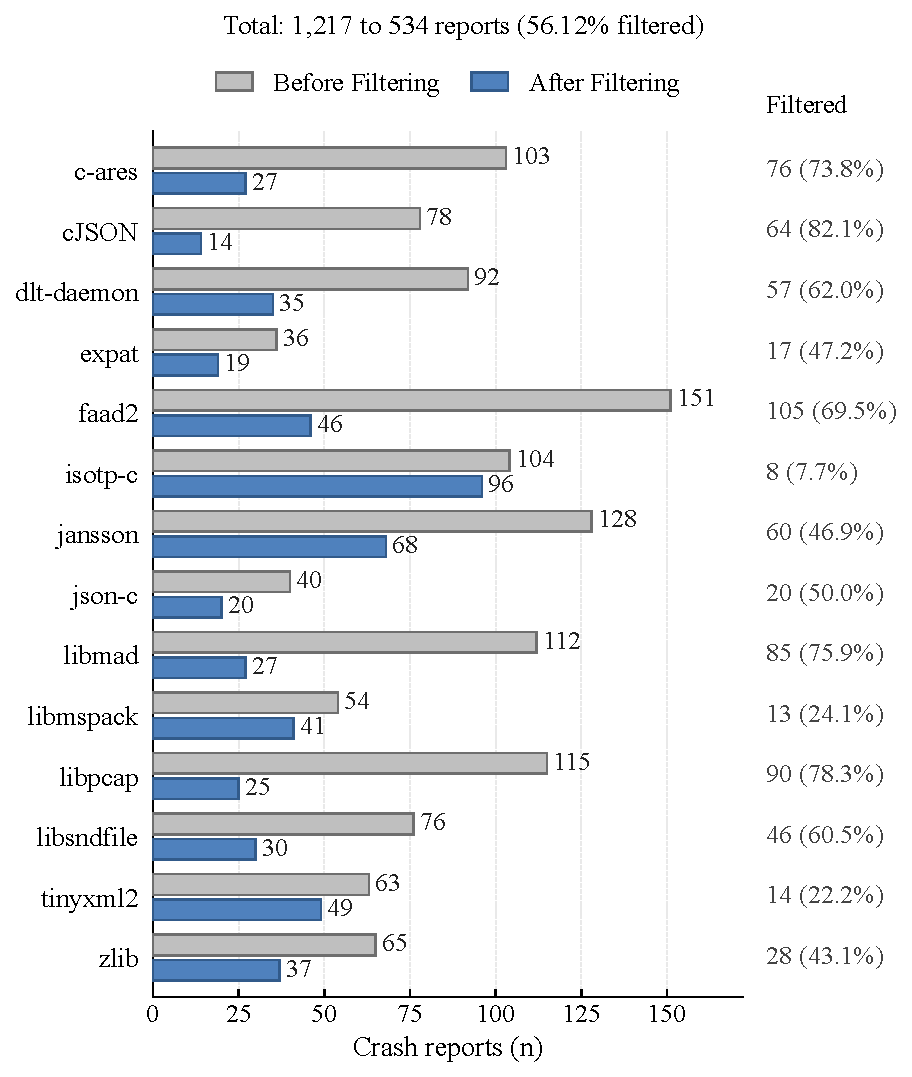
\includegraphics[width=0.75\linewidth]{figures/fig3.pdf}
\caption{Reduction in crash reports after rule-guided crash attribution.}
\label{fig:rule-guided-filtering}
\end{figure}

\begin{table}[!htbp]
\caption{Ground-truth audit of rule-guided filtering.}
\label{tab:filter-safety-audit}
\centering
\color{yellow}
\small
\setlength{\tabcolsep}{3pt}
\renewcommand{\arraystretch}{1.12}
\begin{tabular*}{\linewidth}{@{\extracolsep{\fill}}lccc}
\toprule
Triage Outcome & Ground-truth True & Ground-truth False & Total \\
\midrule
\texttt{noise} & 0 & 103 & 103 \\
\texttt{likely\_driver\_bug} & 0 & 580 & 580 \\
Filtered & 0 & 683 & 683 \\
Retained & 215 & 319 & 534 \\
\botrule
\end{tabular*}
\end{table}

{\color{yellow}
The filtered and retained rows together cover all 1,217 reports; the final target/non-target distribution is reported in Table~\ref{tab:ground-truth-accounting}.
}

\begin{table}[!htbp]
\caption{Effect of rule-guided crash attribution.}
\label{tab:rule-attribution-effect}
\centering
\color{yellow}
\small
\setlength{\tabcolsep}{3pt}
\renewcommand{\arraystretch}{1.12}
\begin{tabular*}{\linewidth}{@{\extracolsep{\fill}}lcccccccc}
\toprule
Variant & LLM Calls & TP & FP & TN & FN & Precision & Recall & F1 \\
\midrule
V0 & 1,217 & 151 & 385 & 617 & 64 & 0.2817 & 0.7023 & 0.4021 \\
V1 & 534 & 155 & 108 & 894 & 60 & 0.5894 & 0.7209 & 0.6485 \\
\botrule
\end{tabular*}
\end{table}

{\color{yellow}
The experimental results are shown in Figure~\ref{fig:rule-guided-filtering} and Tables \ref{tab:filter-safety-audit}, \ref{tab:rule-attribution-effect}, and \ref{tab:per-library-rule-attribution}. Rule-guided crash attribution filters 683 of the 1,217 crash reports and retains 534 reports for subsequent analysis. All 215 confirmed target reports remain in the retained set. The number of LLM submissions therefore decreases from 1,217 to 534.

V0 and V1 use different report populations and different inputs. V0 uses the raw crash report. V1 uses the normalized crash report, triage labels, and matched-rule evidence. The full-population comparison captures the combined effect of report filtering and evidence preparation. We also compare both configurations on the same 534 retained reports. As shown in Table~\ref{tab:v0-v1-decomposition}, V1 identifies more confirmed target reports than V0 on this common population. These results show that rule-guided attribution reduces the analysis workload while retaining all confirmed target reports. They also show that V1 prepares structured evidence for the later context-reconstruction and final-prompt stages. The effects of these stages are evaluated separately in the V2--V3 and V3--V4 comparisons.
}

\begin{table}[!htbp]
\caption{{\color{yellow}V0--V1 comparison on the retained population.}}
\label{tab:v0-v1-decomposition}
\centering
\color{yellow}
\small
\setlength{\tabcolsep}{3pt}
\renewcommand{\arraystretch}{1.12}
\begin{tabularx}{\linewidth}{Y cccc}
\toprule
Configuration & Reports & Precision & Recall & F1 \\
\midrule
V0 predictions on V1-retained reports & 534 & 0.6537 & 0.7023 & 0.6771 \\
V1 on V1-retained reports & 534 & 0.5894 & 0.7209 & 0.6485 \\
\botrule
\end{tabularx}
\end{table}

\begin{table}[!htbp]
\caption{Per-library effect of rule-guided crash attribution.}
\label{tab:per-library-rule-attribution}
\centering
\color{yellow}
\small
\setlength{\tabcolsep}{3pt}
\renewcommand{\arraystretch}{1.12}
\begin{tabular*}{\linewidth}{@{\extracolsep{\fill}}lcccccc}
\toprule
Library & \multicolumn{3}{c}{V0} & \multicolumn{3}{c}{V1} \\
\cmidrule(lr){2-4}\cmidrule(lr){5-7}
& Prec. & Recall & F1 & Prec. & Recall & F1 \\
\midrule
c-ares & 0.1290 & 1.0000 & 0.2286 & 0.5000 & 1.0000 & 0.6667 \\
cJSON & 0.0476 & 0.3333 & 0.0833 & 0.0000 & 0.0000 & 0.0000 \\
dlt-daemon & 0.7442 & 0.9143 & 0.8205 & 1.0000 & 1.0000 & 1.0000 \\
expat & 0.6250 & 0.3846 & 0.4762 & 0.6667 & 0.1538 & 0.2500 \\
faad2 & 0.2267 & 0.5667 & 0.3238 & 0.8947 & 0.5667 & 0.6939 \\
isotp-c & 0.2857 & 0.7500 & 0.4138 & 0.1951 & 1.0000 & 0.3265 \\
jansson & 0.2105 & 0.9231 & 0.3429 & 0.4000 & 0.9231 & 0.5581 \\
json-c & 0.0000 & 0.0000 & 0.0000 & 0.0000 & 0.0000 & 0.0000 \\
libmad & 0.1757 & 1.0000 & 0.2989 & 1.0000 & 1.0000 & 1.0000 \\
libmspack & 0.5667 & 0.9444 & 0.7083 & 1.0000 & 0.8333 & 0.9091 \\
libpcap & 0.4000 & 0.7368 & 0.5185 & 0.8421 & 0.8421 & 0.8421 \\
libsndfile & 0.4545 & 0.3846 & 0.4167 & 0.5200 & 1.0000 & 0.6842 \\
tinyxml2 & 0.3939 & 1.0000 & 0.5652 & 0.5000 & 1.0000 & 0.6667 \\
zlib & 0.3889 & 0.5385 & 0.4516 & 0.2143 & 0.2308 & 0.2222 \\
\botrule
\end{tabular*}
\end{table}
\FloatBarrier

{\color{yellow}
The per-library tables report Precision, Recall, and F1 on the final 1,217 reports. Aggregate improvements do not imply monotonic gains for every library. We retain the project-level results to expose this variability, while the aggregate metrics summarize performance over the full report population.
}

This result is partly attributable to the reports removed by rule-guided crash attribution. Reports with insufficient crash evidence or evidence more consistent with driver-induced failures can introduce misleading information into subsequent analysis. Filtering these reports reduces driver-side cases entering later LLM analysis while preserving target-component candidates that warrant further analysis. In response to RQ1, rule-guided crash attribution distinguishes driver-induced crashes from confirmed-target crashes under the ground-truth labels.

\subsection{Evaluation of Representative Selection}
\label{subsec:representative-evaluation}

To evaluate the efficiency of representative selection, we compare V1 and V2. Both variants apply rule-guided crash attribution to the same crash reports. V1 submits all reports retained after rule-guided crash attribution to the LLM, whereas V2 further applies representative selection before LLM analysis. We first report the runtime of the stages relevant to this comparison and then quantify the reduction in LLM submissions introduced by representative selection.

{\color{yellow}
Table~\ref{tab:stage-latency} reports the mean processing time per sample for crash-context reconstruction and LLM analysis alongside the lightweight report-processing stages. Reconstruction includes seed recovery and binary resolution, static context extraction, direct replay, and Docker/GDB context collection. Seed recovery locates the archived crashing input, while binary resolution identifies its corresponding executable. These four substeps take 0.18 ms, 1.18 ms, 2.44 s, and 18.96 s on average, respectively. Mean context reconstruction time is 21.72 s, with Docker/GDB collection being the dominant substep. Mean LLM analysis latency is 6.63 s. Context measurements were collected serially, with up to three replay/debugger attempts and a 15 s per-attempt timeout. Failed and timed-out attempts are included.
}

\begin{table}[!htbp]
\caption{Mean runtime per sample for the analysis stages.}
\label{tab:stage-latency}
\centering
\color{yellow}
\small
\setlength{\tabcolsep}{3pt}
\renewcommand{\arraystretch}{1.12}
\begin{tabularx}{\linewidth}{Y L{0.24\linewidth} C{0.21\linewidth}}
\toprule
Stage & Samples & Mean time per sample \\
\midrule
Sanitizer parsing & 1,217 reports & 0.67 ms \\
Rule-guided attribution & 1,217 reports & 0.10 ms \\
Representative selection & 534 retained reports & 0.01 ms \\
Seed recovery and binary resolution & 96 representatives & 0.18 ms \\
Static context extraction & 96 representatives & 1.18 ms \\
Direct replay & 96 representatives & 2.44 s \\
Docker/GDB context collection & 96 representatives & 18.96 s \\
Context reconstruction (overall) & 96 representatives & 21.72 s \\
Evidence packaging and prompt construction & 96 representatives & 0.34 s \\
LLM analysis & 96 representatives & 6.63 s \\
End-to-end representative analysis & 96 representatives & 28.69 s \\
\botrule
\end{tabularx}
\end{table}

{\color{yellow}
The mean end-to-end latency across the 96 representative samples is 28.69 s, covering context reconstruction, evidence packaging and prompt construction, and LLM analysis. Context and prompt times come from the timing measurements, while LLM latency comes from the archived responses for the same representatives.

The evaluated target API sets range from 12 to 60. cJSON (60 APIs) and libpcap (30 APIs) both reduce their respective sets of 78 and 115 reports to four LLM submissions, with mean LLM latencies of 6.17 s and 6.23 s per representative. In comparison, faad2 (12 APIs) reduces 151 reports to nine submissions, with a mean LLM latency of 7.72 s. Across all 14 libraries, project-level mean LLM latency ranges from 5.52 s to 7.72 s. These results support the potential scalability of representative-based, crash-local analysis to untested libraries with larger API sets. The analysis workload for such libraries would depend on representative count and per-representative replay/debugger cost.
}

\begin{figure}[H]
\centering
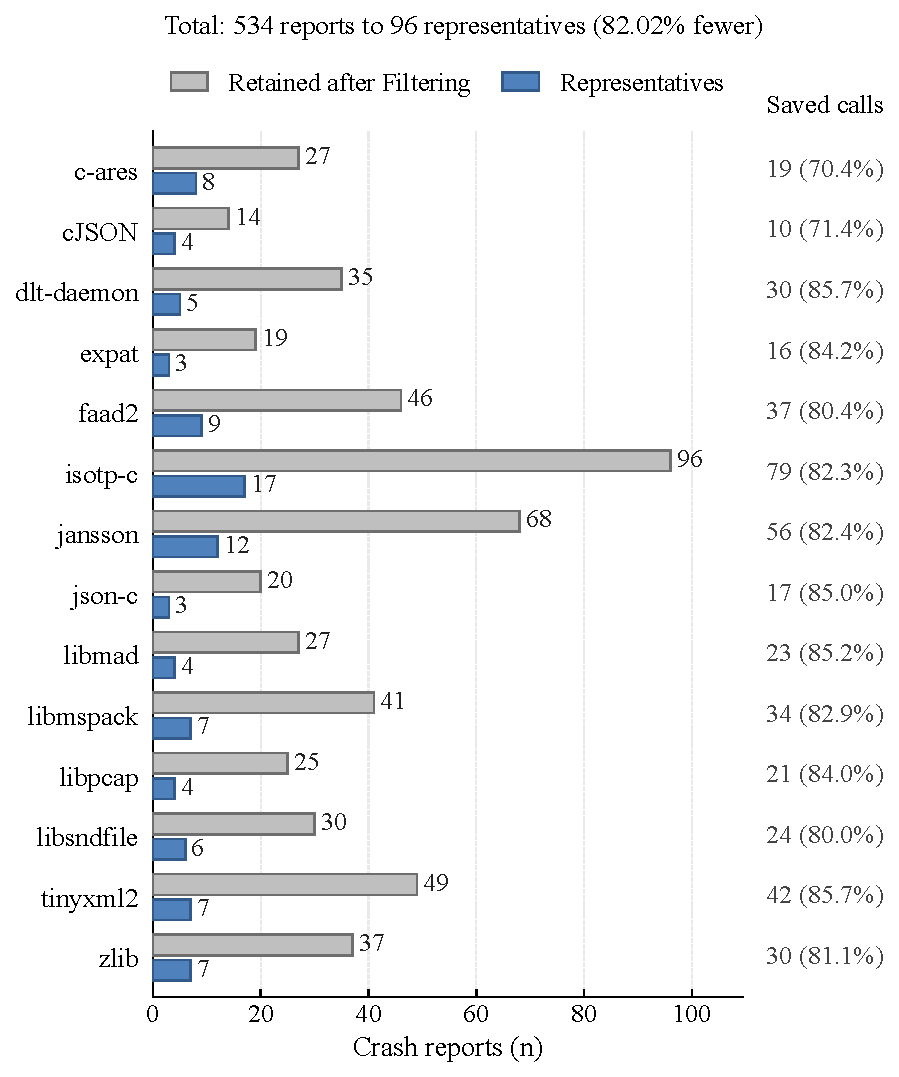
\includegraphics[width=0.75\linewidth]{figures/fig4.pdf}
\caption{Reduction in {\color{yellow}crash reports} achieved by representative selection.}
\label{fig:representative-counts}
\end{figure}

{\color{yellow}
On the final 1,217-report dataset, rule-guided attribution retains 534 reports, and representative selection reduces this set to 96 representatives, a reduction of 82.02\% relative to the retained workload. Only the prediction of each representative is propagated through the saved mapping. Every report retains its own ground-truth label, and TP, FP, TN, and FN are computed against that label. To evaluate group-level error propagation, we flip each representative prediction individually and recompute the report-level metrics. The maximum absolute F1 change is 0.0174; the worst-case flip reduces F1 from 0.8379 to 0.8205 and affects less than 1\% of report-level decisions.
}

{\color{yellow}
To compare representative selection directly, we apply ReBucket to the same 534 reports retained after rule-guided attribution. CrashSage selects 96 representatives, whereas ReBucket selects 103 cluster representatives, corresponding to reductions of 82.02\% and 80.71\%, respectively. Thus, ReBucket requires seven additional LLM submissions relative to CrashSage on this workload. At the pairwise level, ReBucket preserves 1,450 of the 1,476 report pairs that CrashSage groups together and splits the remaining 26 pairs.
}

\begin{table}[!htbp]
\caption{{\color{yellow}Representative-selection comparison on the same retained reports.}}
\label{tab:rebucket-comparison}
\centering
\color{yellow}
\small
\setlength{\tabcolsep}{3pt}
\renewcommand{\arraystretch}{1.12}
\begin{tabular*}{\linewidth}{@{\extracolsep{\fill}}lccc}
\toprule
Method & Retained reports & Representatives & Reduction \\
\midrule
CrashSage & 534 & 96 & 82.02\% \\
ReBucket & 534 & 103 & 80.71\% \\
\botrule
\end{tabular*}
\end{table}

{\color{yellow}
Figure~\ref{fig:rebucket-representative-selection} presents ReBucket's retained reports and representatives for each library in the same format as the CrashSage results. The representative counts differ for cJSON, with 4 for CrashSage and 9 for ReBucket, and libpcap, with 4 and 6, respectively. The other 12 libraries have the same representative counts under both methods. Each reduction is computed relative to that library's retained reports.
}

\begin{figure}[H]
\centering
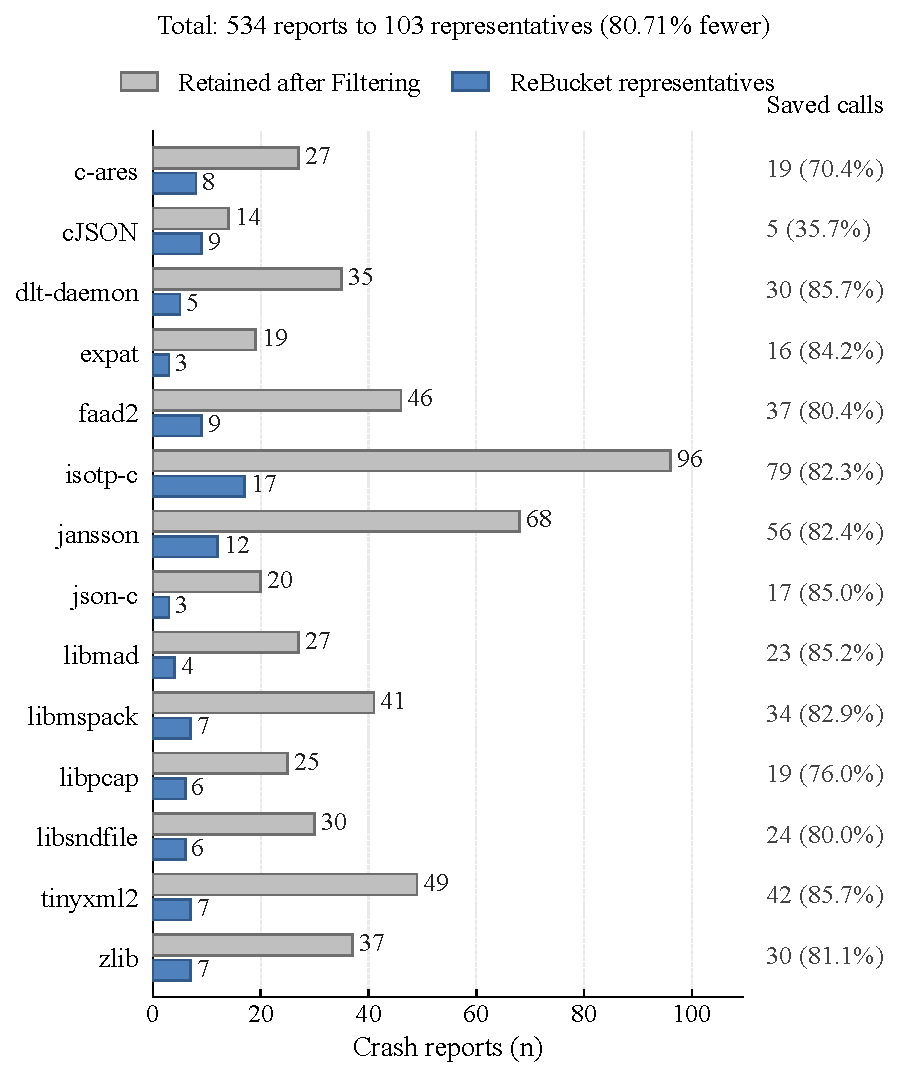
\includegraphics[width=0.75\linewidth]{figures/fig4_rebucket.pdf}
\caption{Per-library representative selection with ReBucket on the same retained reports. Gray bars show the reports retained after filtering, and blue bars show the ReBucket representatives. The right column reports the number and percentage of saved LLM submissions.}
\label{fig:rebucket-representative-selection}
\end{figure}

\begin{table}[!htbp]
\caption{{\color{yellow}Pairwise agreement between CrashSage and ReBucket.}}
\label{tab:rebucket-pairwise}
\centering
\color{yellow}
\small
\setlength{\tabcolsep}{3pt}
\renewcommand{\arraystretch}{1.12}
\begin{tabular*}{\linewidth}{@{\extracolsep{\fill}}lc}
\toprule
Metric & Count \\
\midrule
Shared co-clustered report pairs & 1,450 \\
Report pairs co-clustered by CrashSage only & 26 \\
Report pairs co-clustered by ReBucket only & 0 \\
Pairwise Jaccard agreement & 0.9824 \\
\botrule
\end{tabular*}
\end{table}

{\color{yellow}
We audit whether representative selection merges distinct confirmed targets in two complementary views. The structural audit covers all 215 confirmed-target reports and groups them by project, sanitizer bug type, first target-project frame, and crash function. The CVE audit covers the 80 reports with explicit public CVE identifiers. As summarized below, neither audit merges distinct confirmed targets, and all target and CVE categories remain represented after selection.
}

\begin{table}[!htbp]
\caption{{\color{yellow}Confirmed-target consistency after representative selection.}}
\label{tab:target-consistency}
\centering
\color{yellow}
\small
\setlength{\tabcolsep}{3pt}
\renewcommand{\arraystretch}{1.12}
\begin{tabularx}{\linewidth}{Y c C{0.15\linewidth} C{0.23\linewidth} C{0.12\linewidth} C{0.11\linewidth}}
\toprule
Audit scope & Reports & Representative groups & Reference classes & Mixed-class groups & Classes retained \\
\midrule
All confirmed targets & 215 & 42 & 16 structural fingerprints & 0 & 16/16 \\
Explicit public-CVE subset & 80 & 19 & 7 CVEs & 0 & 7/7 \\
\botrule
\end{tabularx}
\end{table}

{\color{yellow}
The structural fingerprint is an auditable crash-site proxy rather than an independent manual root-cause label. The 80 CVE-linked reports are a subset of the 215 confirmed targets; the remaining 135 reports comprise 66 author-confirmed public driver+PoC cases without a CVE identifier, 43 targets from dlt-daemon and isotp-c, and 26 targets from the completed audit.
}

The reduction varies across libraries because the generated crashing inputs contain different levels of repetition. In response to RQ2, representative selection reduces repeated LLM analysis over the retained reports by keeping one report for each group of crashes with matching exact or stack signatures.

\subsection{Evaluation of Crash-Context Reconstruction}
\label{subsec:rq3-localization}

To evaluate crash-context reconstruction, we compare V2 and V3 on the same {\color{yellow}1,217} crash reports. Both variants use rule-guided crash attribution and representative selection, while only V3 includes crash-context reconstruction. With the ground-truth labels held fixed, this comparison evaluates the effect of adding crash-context reconstruction to V2.

\begin{table}[!htbp]
\caption{Effect of crash-context reconstruction.}
\label{tab:context-effect-v2-v3}
\centering
\color{yellow}
\small
\setlength{\tabcolsep}{3pt}
\renewcommand{\arraystretch}{1.12}
\begin{tabular*}{\linewidth}{@{\extracolsep{\fill}}lcccccccc}
\toprule
Variant & LLM Calls & TP & FP & TN & FN & Precision & Recall & F1 \\
\midrule
V2 & 96 & 155 & 108 & 894 & 60 & 0.5894 & 0.7209 & 0.6485 \\
V3 & 96 & 186 & 75 & 927 & 29 & 0.7126 & 0.8651 & 0.7815 \\
\botrule
\end{tabular*}
\end{table}

{\color{yellow}
On the same 1,217 reports, adding crash-context reconstruction raises F1 from 0.6485 in V2 to 0.7815 in V3. TP increases from 155 to 186, FP decreases from 108 to 75, and FN decreases from 60 to 29. Static context links the visible crash site to the driver-to-component call path, while runtime context records the state observed during replay. Together, these evidence sources support attribution by distinguishing the visible crash location from the origin of the faulty state.
}

\begin{table}[!htbp]
\caption{Per-library effect of crash-context reconstruction.}
\label{tab:per-library-context-reconstruction}
\centering
\color{yellow}
\small
\setlength{\tabcolsep}{3pt}
\renewcommand{\arraystretch}{1.12}
\begin{tabular*}{\linewidth}{@{\extracolsep{\fill}}lcccccc}
\toprule
Library & \multicolumn{3}{c}{V2} & \multicolumn{3}{c}{V3} \\
\cmidrule(lr){2-4}\cmidrule(lr){5-7}
& Prec. & Recall & F1 & Prec. & Recall & F1 \\
\midrule
c-ares & 0.5000 & 1.0000 & 0.6667 & 0.5000 & 1.0000 & 0.6667 \\
cJSON & 0.0000 & 0.0000 & 0.0000 & 0.0000 & 0.0000 & 0.0000 \\
dlt-daemon & 1.0000 & 1.0000 & 1.0000 & 1.0000 & 1.0000 & 1.0000 \\
expat & 0.6667 & 0.1538 & 0.2500 & 0.0000 & 0.0000 & 0.0000 \\
faad2 & 0.8947 & 0.5667 & 0.6939 & 1.0000 & 1.0000 & 1.0000 \\
isotp-c & 0.1951 & 1.0000 & 0.3265 & 0.5333 & 1.0000 & 0.6957 \\
jansson & 0.4000 & 0.9231 & 0.5581 & 0.3824 & 1.0000 & 0.5532 \\
json-c & 0.0000 & 0.0000 & 0.0000 & 0.6500 & 1.0000 & 0.7879 \\
libmad & 1.0000 & 1.0000 & 1.0000 & 1.0000 & 1.0000 & 1.0000 \\
libmspack & 1.0000 & 0.8333 & 0.9091 & 1.0000 & 1.0000 & 1.0000 \\
libpcap & 0.8421 & 0.8421 & 0.8421 & 0.6667 & 0.6316 & 0.6486 \\
libsndfile & 0.5200 & 1.0000 & 0.6842 & 0.8667 & 1.0000 & 0.9286 \\
tinyxml2 & 0.5000 & 1.0000 & 0.6667 & 0.3571 & 0.7692 & 0.4878 \\
zlib & 0.2143 & 0.2308 & 0.2222 & 0.6842 & 1.0000 & 0.8125 \\
\botrule
\end{tabular*}
\end{table}
{\color{yellow}
The project-level effects vary. For example, json-c increases from F1 0.0000 in V2 to 0.7879 in V3, while cJSON remains at 0.0000. The next subsection holds the reconstructed evidence fixed and examines how final-prompt design affects the representative decisions.
}
\FloatBarrier
\subsection{Evaluation of Final-Prompt Sensitivity and LLM}
\label{subsec:rq4-sensitivity}

{\color{yellow}
To identify which part of the differential prompt contributes to the improvement, we compare four nested prompt variants on the same representatives and the same evidence package. P0 is the Clean direct prompt used in V3. P1 adds the two-hypothesis comparison, P2 adds the precondition check and \texttt{evidence\_rationale}, and P3 adds the boundary rules used in V4.
}

\begin{table}[!htbp]
\caption{{\color{yellow}Nested prompt ablation on 1,217 crash reports.}}
\label{tab:prompt-form-ablation}
\centering
\color{yellow}
\small
\setlength{\tabcolsep}{3pt}
\renewcommand{\arraystretch}{1.12}
\begin{tabular*}{\linewidth}{@{\extracolsep{\fill}}lccc}
\toprule
Prompt & Precision & Recall & F1 \\
\midrule
P0 (V3) & 0.7126 & 0.8651 & 0.7815 \\
P1 & 0.7263 & 0.9256 & 0.8139 \\
P2 & 0.7453 & 0.9256 & 0.8257 \\
P3 (V4) & 0.7654 & 0.9256 & 0.8379 \\
\botrule
\end{tabular*}
\end{table}

{\color{yellow}
Table~\ref{tab:prompt-form-ablation} shows that F1 rises at every step. The three steps do not act on the same error type. P1 is the only step that recovers missed target-component crashes, and recall stops rising after it. P2 and P3 recover no further true positives and remove false positives only, so precision keeps rising while recall stays fixed. The hypothesis comparison is therefore the component that governs recall, and the two later components refine precision. The benefit of the differential prompt comes from this separation rather than from a single template change.

Table~\ref{tab:per-library-final-prompt} reports the same comparison per project. Only cJSON, expat, and jansson change between V3 and V4; the other eleven projects are unchanged. cJSON and expat gain target attributions, while jansson improves precision with recall already at 1.0000.
}

\begin{table}[!htbp]
\caption{{\color{yellow}Per-library effect of final prompt design under Qwen3-Coder-Flash.}}
\label{tab:per-library-final-prompt}
\centering
\color{yellow}
\small
\setlength{\tabcolsep}{3pt}
\renewcommand{\arraystretch}{1.12}
\begin{tabular*}{\linewidth}{@{\extracolsep{\fill}}lcccccc}
\toprule
Library & \multicolumn{3}{c}{V3} & \multicolumn{3}{c}{V4} \\
\cmidrule(lr){2-4}\cmidrule(lr){5-7}
& Prec. & Recall & F1 & Prec. & Recall & F1 \\
\midrule
c-ares & 0.5000 & 1.0000 & 0.6667 & 0.5000 & 1.0000 & 0.6667 \\
cJSON & 0.0000 & 0.0000 & 0.0000 & 1.0000 & 1.0000 & 1.0000 \\
dlt-daemon & 1.0000 & 1.0000 & 1.0000 & 1.0000 & 1.0000 & 1.0000 \\
expat & 0.0000 & 0.0000 & 0.0000 & 1.0000 & 0.5385 & 0.7000 \\
faad2 & 1.0000 & 1.0000 & 1.0000 & 1.0000 & 1.0000 & 1.0000 \\
isotp-c & 0.5333 & 1.0000 & 0.6957 & 0.5333 & 1.0000 & 0.6957 \\
jansson & 0.3824 & 1.0000 & 0.5532 & 0.6500 & 1.0000 & 0.7879 \\
json-c & 0.6500 & 1.0000 & 0.7879 & 0.6500 & 1.0000 & 0.7879 \\
libmad & 1.0000 & 1.0000 & 1.0000 & 1.0000 & 1.0000 & 1.0000 \\
libmspack & 1.0000 & 1.0000 & 1.0000 & 1.0000 & 1.0000 & 1.0000 \\
libpcap & 0.6667 & 0.6316 & 0.6486 & 0.6667 & 0.6316 & 0.6486 \\
libsndfile & 0.8667 & 1.0000 & 0.9286 & 0.8667 & 1.0000 & 0.9286 \\
tinyxml2 & 0.3571 & 0.7692 & 0.4878 & 0.3571 & 0.7692 & 0.4878 \\
zlib & 0.6842 & 1.0000 & 0.8125 & 0.6842 & 1.0000 & 0.8125 \\
\botrule
\end{tabular*}
\end{table}

{\color{yellow}
The cJSON result illustrates how representative-level decisions translate into report-level metrics. Its 78 reports contain six target and 72 non-target reports. Filtering retains 14 reports, which map to four representatives; all six target reports share one representative. With the evidence package and mapping fixed, this representative changes from non-target under V3 to target under V4, and its prediction is propagated to the six group members. The remaining 72 reports keep their non-target decisions. Consequently, TP changes from 0 to 6 and FN from 6 to 0, while FP remains 0 and TN remains 72, yielding the F1 change from 0.0000 to 1.0000. In the P1 configuration reported in the component-ablation table, the same representative already changes to target after the two-hypothesis comparison is added. Thus, the large project-level change reflects a prompt-sensitive representative decision shared by all six positives, rather than six independent model decisions.
}

{\color{yellow}
Run-to-run stability. The four prompt configurations defined in the prompt-component ablation were frozen before evaluation and shared across projects. No project names, expected CVE identifiers, or ground-truth labels were inserted into the templates. We repeated each configuration six times at temperature 0 and report decision variability at both the run and report levels. The main table uses the formal V3/V4 endpoints for P0/P3 and the median-F1 runs recorded in the experiment manifest for P1/P2; both selected intermediate runs are run1. The P2 and P3 intervals overlap, so their difference is interpreted as an observed effect rather than a statistically significant improvement.
}

\begin{table}[!htbp]
\caption{{\color{yellow}Six-run stability of the nested prompt ablation.}}
\label{tab:prompt-run-stability}
\centering
\color{yellow}
\small
\setlength{\tabcolsep}{3pt}
\renewcommand{\arraystretch}{1.12}
\begin{tabularx}{\linewidth}{l c c Y C{0.23\linewidth}}
\toprule
Prompt & Mean F1 & SD & 95\% run-bootstrap interval & Reports changed across runs \\
\midrule
P0 & 0.7788 & 0.0051 & [0.7741, 0.7815] & 9 / 1,217 \\
P1 & 0.8095 & 0.0063 & [0.8046, 0.8139] & 13 / 1,217 \\
P2 & 0.8260 & 0.0100 & [0.8178, 0.8342] & 14 / 1,217 \\
P3 & 0.8295 & 0.0085 & [0.8220, 0.8355] & 23 / 1,217 \\
\botrule
\end{tabularx}
\end{table}

{\color{yellow}
The repeated results therefore show limited report-level variation even at temperature 0. Full precision, recall, per-run values, and bootstrap settings are provided in the supplementary result record.
}


{\color{yellow}
CrashSage-V4 outperforms V3 on the same 1,217 crash reports; the quantitative comparison is reported in the main ablation table.

Furthermore, to evaluate whether the effectiveness of CrashSage-V4 depends on the final LLM backend, we repeat the V4 experiment with five additional LLMs. The representative crashes, reconstructed contexts, V4 prompt configuration, representative mapping, and ground-truth labels are held fixed; only the final LLM is replaced. All models are evaluated at temperature 0 on the same 96 representatives, and the decisions are expanded to the same 1,217 crash reports.

The primary CrashSage-V4 model is \texttt{qwen3-coder-flash}, accessed on 1 November 2026 through the OpenAI-compatible endpoint \url{https://llm-1aqn2a1i6uz9t6gu.cn-beijing.maas.aliyuncs.com/compatible-mode/v1}. This model was selected on four engineering metrics: general and code-analysis capability, long-context capacity, service stability and response latency, and API cost.

The alternative backends are \texttt{qwen-flash}, \texttt{qwen3.8-flash}, \texttt{deepseek-flash}, \texttt{gpt-5.6-sol}, and \texttt{glm-5.3-flash}, accessed between 30 October and 1 November 2026. Each backend was accessed through the API provider under its exact model identifier. We report the model identifiers and access dates and retain the corresponding model responses in the experiment archive. All configurations use \texttt{temperature=0}.
}

\begin{table}[!htbp]
\caption{{\color{yellow}Effect of the final LLM backend under V4. All configurations use the same V4 setting and are evaluated on 1,217 crash reports; only the final LLM is changed.}}
\label{tab:llm-model-ablation}
\centering
\color{yellow}
\small
\setlength{\tabcolsep}{3pt}
\renewcommand{\arraystretch}{1.12}
\begin{tabularx}{\linewidth}{Y ccc}
\toprule
LLM Backend & Precision & Recall & F1 \\
\midrule
Qwen3-Coder-Flash (default V4) & 0.7654 & 0.9256 & 0.8379 \\
Qwen-Flash & 0.7425 & 0.9256 & 0.8240 \\
Qwen3.8-Flash & 0.7636 & 0.9163 & 0.8330 \\
DeepSeek-Flash & 0.7645 & 0.9209 & 0.8354 \\
GPT-5.6-Sol & 0.7645 & 0.9209 & 0.8354 \\
GLM-5.3-Flash & 0.7606 & 0.9163 & 0.8312 \\
\botrule
\end{tabularx}
\end{table}

{\color{yellow}
The evaluated backends achieve closely matched overall performance, indicating that the observed V4 behavior is consistent across the evaluated backend choices. Backend selection can therefore follow deployment requirements while preserving the overall method behavior.
}

\FloatBarrier

\subsection{Case Studies}
\label{subsec:case-studies}

To complement the quantitative results above, we present three case studies that illustrate how CrashSage prepares structured crash evidence before final LLM analysis. They are selected to match the three evaluation concerns studied above: false-alert judgment, efficiency, and crash localization.

Table~\ref{tab:case-study-evidence} summarizes three case studies corresponding to the three evaluation concerns. In Case 1, the sanitizer reports a \texttt{heap-buffer-overflow}, but the top crashing frame and heap-boundary evidence are both confined to the generated driver.
The driver allocates a 20-byte \texttt{second\_str} buffer and then writes the terminator after copying fuzz input into that buffer, so the faulty state is created before any target-component behavior needs to be considered.
CrashSage therefore treats this report as \texttt{likely\_driver\_bug} and filters it before LLM analysis, illustrating how rule-guided attribution prevents a driver memory error from being counted as a target-component crash candidate.

In Case 2, the libpcap reports form a repeated SEGV group rather than independent failures. The raw reports share similar crash-site evidence and stack signatures, and CrashSage records repeated reports in the \texttt{driver\_30} group as duplicates of selected representative reports.
Representative selection therefore skips duplicate LLM submissions and reuses the representative mapping, providing a concrete instance of the RQ2 result: redundant SEGV reports are collapsed by signature evidence before final analysis.

\begin{table}[ht]
\caption{Case studies for CrashSage evaluation}
\label{tab:case-study-evidence}
\centering
\compacttable
\setlength{\tabcolsep}{2.6pt}
\renewcommand{\arraystretch}{1.12}
\begin{tabularx}{\linewidth}{L{0.15\linewidth} Y Y Y}
\toprule
Evidence &
Case 1: False-alert judgment &
Case 2: Efficiency &
Case 3: Crash localization \\
\midrule
Crash report
& cJSON \texttt{driver\_4\_crash\_1}
& libpcap \texttt{driver\_30} group
& json-c \texttt{driver\_13\_crash\_1} \\
\midrule
Failure identity
& \texttt{heap-buffer-overflow}
& repeated \texttt{SEGV}
& \texttt{SEGV} wild write \\
\midrule
Attribution evidence
& top crashing frame: driver
& shared crash-site / stack signature
& project frame in \texttt{printbuf\_memappend} \\
\midrule
Context or mapping
& 20-byte driver heap region
& duplicate--representative pair; 10+ reports
& state-sensitive \texttt{printbuf} context; replay confirmed \\
\midrule
Pipeline output
& \texttt{likely\_driver\_bug}; filtered
& duplicate skipped; representative reused
& context-supported \texttt{is\_api\_bug=true} result \\
\botrule
\end{tabularx}
\end{table}
\FloatBarrier

In Case 3, the raw prompt-based analysis does not return \texttt{is\_api\_bug=true} for the json-c crash, although the crash is labeled true under the ground-truth labels.
CrashSage changes this decision after reconstructing the state-sensitive context around \texttt{printbuf\_memappend}.
The context records that the driver-created \texttt{printbuf} reaches the library with boundary-sensitive position and size fields.
Replay confirms that this state consistently reaches the same failing library path.
The reconstructed data flow shows that the generated driver directly sets \texttt{pb->bpos} near \texttt{INT\_MAX} while keeping \texttt{pb->size} small before invoking \texttt{printbuf\_memappend}.
The additional static and runtime context changes the raw-report-level negative result into an \texttt{is\_api\_bug=true} result consistent with the confirmed-target ground-truth label.

\FloatBarrier

\section{Limitations}
\label{sec:limitations}

{\color{yellow}
The evaluation covers third-party-library components relevant to connected-vehicle software. Its scope is component-level crash adjudication; full vehicle stacks, ECU integration, and on-vehicle deployment remain separate validation settings. The reported results and their applicability are interpreted within this component-level scope.
}

The current implementation follows one LLM-assisted fuzz-driver generation workflow and uses ASan+UBSan instrumentation. This setting is consistent across all evaluated variants, which keeps the comparison controlled, but other driver generators, prompt strategies, fuzzing engines, or sanitizer configurations may change the proportion of driver-induced crashes, duplicate reports, and target-component candidates. Extending CrashSage to additional driver-generation workflows and sanitizer combinations is left as future work.

Rule-guided crash attribution is based on a predefined set of deterministic rules over sanitizer signals and stack-frame roles. These rules are designed to conservatively remove reports with insufficient crash evidence or evidence more consistent with driver-induced failures, but their coverage is still bounded by the sanitizer information and stack structure available in each report. Crash-context reconstruction depends on replaying the crashing input and collecting runtime state in a stable execution environment. When replay fails or the reproduced crash does not match the original signature, CrashSage falls back to the normalized crash report and static context, which may reduce localization confidence. Different LLM capabilities or false-alert ratios may change the observed gains. CrashSage is therefore most appropriate as an evidence-preparation and attribution aid: it preserves reports that warrant further analysis and records the evidence used for each filtering or retention decision.

\FloatBarrier

\section{Conclusion}
\label{sec:conclusion}

{\color{yellow}
CrashSage introduces an evidence-guided crash-adjudication pipeline for LLM-assisted fuzzing of third-party open-source libraries. Rule-guided attribution, representative selection, and crash-context reconstruction prepare filtered, representative, and localized evidence before final LLM analysis. Evaluation on 1,217 crash reports from 14 libraries relevant to connected-vehicle software yields 76.54\% precision, 92.56\% recall, and an 83.79\% F1 score. Filtering retains 534 reports, and representative selection reduces this workload to 96 representatives, requiring 92.11\% fewer LLM submissions than analysis of all 1,217 reports. Runtime measurements show that context reconstruction and LLM analysis dominate the cost. The mean end-to-end latency across the 96 representative samples is 28.69 s. These results support CrashSage as a component-level crash-attribution aid in the connected-vehicle application setting. Future work will extend evaluation to additional driver-generation workflows and sanitizer configurations.
}

\backmatter

\bmhead{Acknowledgements}

Not applicable.

\bmhead{Authors' contributions}

Gaoqing Guan contributed to conceptualization, methodology, implementation, evaluation, and writing of the original draft. Ying Zhang, Letian Sha, and Huiran Yang contributed to experimental design, validation, result analysis and interpretation, and manuscript review and editing. All authors read and approved the final manuscript.

\bmhead{Funding}

Not applicable.

\bmhead{Availability of data and materials}

The data supporting the findings of this study are available from the corresponding author upon reasonable request.

\section*{Declarations}

\bmhead{Competing interests}

The authors declare that they have no known competing financial interests or personal relationships that could have appeared to influence the work reported in this paper.

% ================= References =================
\bibliography{sn-bibliography}

\end{document}
